\documentclass[12pt,a4paper]{article}
\usepackage[utf8]{inputenc}
\usepackage[T1]{fontenc}
\usepackage{amsmath,amssymb,amsthm}
\usepackage{geometry}
\usepackage{booktabs}
\usepackage{hyperref}
\usepackage{longtable}
\usepackage{pdflscape}
\usepackage{array}
\usepackage{tikz}
\usepackage{pgfplots}
\pgfplotsset{compat=1.18}
\usepackage{graphicx}
\usepackage{float}
\usepackage[font=small,labelfont=bf]{caption}

\geometry{margin=1.1in}

\newtheorem{theorem}{Theorem}[section]
\newtheorem{lemma}[theorem]{Lemma}
\newtheorem{corollary}[theorem]{Corollary}

\theoremstyle{definition}
\newtheorem{definition}[theorem]{Definition}

\theoremstyle{remark}
\newtheorem{remark}[theorem]{Remark}

\hypersetup{colorlinks=true, linkcolor=blue, urlcolor=blue, citecolor=blue}

\title{The Geometric Computer:\\
Turing Completeness, Free Energy, and Learning\\
in a Digital Brain on $S^3$}

\author{
Walter Henrique Alves da Silva\\
\texttt{walter.h057@gmail.com}\quad
ORCID: 0009-0001-0857-096X\\[4pt]
Open Research Institute
}

\date{April 2026}

\begin{document}

\maketitle

\begin{abstract}
In 1948 Shannon recognized that thermodynamic entropy and minimum description
length are the same function, and that recognition unified physics and
information theory. This paper makes the same move for the geometry of
computation.

The function $\sigma(\mathrm{compose}(A, \mathrm{inverse}(B)))$ --- the
geodesic distance from the ground state on the unit 3-sphere $S^3$ --- is
the entropy of geometric computation. It is simultaneously the Free Energy
Principle's prediction error (exact, because the state space is $S^3$), the
proximity measure for Riemann non-trivial zeros, the branch-on-zero condition
of any Turing-complete counter machine, and the opponent-channel structure
of human trichromatic vision. These are identities, and the list extends to
every discipline that has a ground state.

From this distance, a complete digital brain is derived: perception,
evaluation, three-layer topological memory, resonance-based attention,
hierarchical abstraction, affect, neuromodulation, and self-observation ---
all from one arithmetic operation, the Hamilton product on $S^3$. The
brain is Turing-complete by construction, learns in one pass, and
self-monitors through a geometric observable that is the exact Free Energy
Principle on a compact Lie group. The architecture is a new computing
paradigm: the first computer where the state space is $\mathrm{SU}(2)$
--- the quantum gate group --- making quantum computation native to the
substrate, and the first whose computational primitives are identical to
those of biological neural oscillators. The system runs in production, 
every constant is derived from topology, every claim is experimentally
verified.
\end{abstract}

\tableofcontents\newpage

% ============================================================
\section{Introduction}
% ============================================================

Shannon's 1948 paper recognized that two fields --- thermodynamics and
communication --- were measuring the same quantity under different names,
and that recognition unified them. The entropy $H = -\sum p \log p$ was
already known to Boltzmann; Shannon identified it as the minimum
description length of a message source.  Same math, read from
a different angle, connected two sciences.

This paper makes the same move for geometry, and the consequences are
larger, because the function that unifies is also the function that
computes. The measurement

\[
  \sigma(\mathrm{compose}(A, \mathrm{inverse}(B)))
\]

is the geodesic distance from the ground state on the unit 3-sphere $S^3$.
Every discipline that has a ground state measures this distance under its
own name: arithmetic calls it error, neuroscience calls it prediction error,
number theory calls it distance from the critical line, and vision calls it
opponent-channel imbalance. One function, one space, and the list extends
to every system that can be in or out of equilibrium --- which is every
system.

The function is also computable: The Hamilton product of two unit quaternions
on $S^3$ is a single fixed-point arithmetic operation (four floats in, four
floats out), and from this one operation a complete digital brain is derived:
perception, memory, learning, attention, consolidation, affect, hierarchy,
and self-observation. The brain is Turing-complete, learns associations in
one pass, runs the Free Energy Principle exactly, reproduces human
trichromatic vision as a structural consequence of the algebra, and observes
its own internal coherence at every step through a geometric signal that
functions as a dopamine analog.

The architecture is implemented in Rust as the \texttt{closure\_ea} crate,
runs in production, and every claim in this paper is verified by one of 13
experiments (Section~\ref{sec:experiments}). Both the implementation and the prior paper
establishing the two axioms~\cite{alves2026zeroth} are public. The machine computes.

What follows is the derivation from first principles. Section~\ref{sec:geometry}
shows why $S^3$ is forced, then derives arithmetic and Turing completeness
from orbits on that manifold. Section~\ref{sec:brain} builds the complete brain
architecture --- learning loop, Free Energy Principle, perception channels,
affect, memory consolidation, and neuromodulation. Section~\ref{sec:consciousness}
shows how the machine observes its own coherence through a geometric signal
that functions as a dopamine analog. Section~\ref{sec:universality} shows what
the same construction produces across number theory, biology, quantum mechanics,
discrete dynamics, and the structure of space-time when the substrate is shared.
Section~\ref{sec:experiments} presents the experimental results. Section~\ref{sec:discussion} traces the implications for hardware,
security, intelligence at the edge, biological interfaces, and coordination
at scale.

Table~\ref{tab:comparison} maps every cognitive and computational function to
its location in the architecture --- and to its analogue in a biological
brain, a Unix kernel, a von Neumann CPU, and a transformer. The purpose is to
show completeness at a glance: no function is missing, and every function is
derived from the same manifold.

\begin{landscape}
\begin{longtable}{>{\bfseries\footnotesize}p{3.0cm}
                  >{\footnotesize}p{3.8cm}
                  >{\footnotesize}p{3.2cm}
                  >{\footnotesize}p{2.8cm}
                  >{\footnotesize}p{3.2cm}
                  >{\footnotesize}p{4.4cm}}
\caption{Every function of the geometric brain, mapped to its analogue in
known systems.}
\label{tab:comparison}\\
\toprule
\textbf{Function} & \textbf{Biological Brain} & \textbf{Unix Kernel} &
\textbf{Von Neumann CPU} & \textbf{Transformer} & \textbf{closure\_ea} \\
\midrule
\endfirsthead
\multicolumn{6}{c}{\tablename~\thetable{} (continued)}\\
\toprule
\textbf{Function} & \textbf{Biological Brain} & \textbf{Unix Kernel} &
\textbf{Von Neumann CPU} & \textbf{Transformer} & \textbf{closure\_ea} \\
\midrule
\endhead
\midrule\multicolumn{6}{r}{\footnotesize(continued on next page)}\\
\endfoot
\bottomrule
\endlastfoot
Input boundary &
  Sensory transduction (photoreceptors $\to$ spikes) &
  \texttt{read(2)} syscall &
  Instruction fetch &
  Tokenizer + embedding &
  \texttt{domain\_embed()}, \texttt{bytes\_to\_sphere4()} $\to$ carrier on $S^3$ \\[4pt]
Transient working space &
  Working memory (prefrontal, $\sim$7 items) &
  Page cache, process stack &
  Registers + cache &
  KV cache (context window) &
  \texttt{Buffer} (rolling transient entries) \\[4pt]
Long-term perceptual memory &
  Neocortical LTP &
  Filesystem (inode tree) &
  Main memory (RAM) &
  Learned weight matrix &
  Genome --- Epigenetic layer \\[4pt]
Structural anchors &
  Brainstem reflex arcs, genetic constraints &
  Kernel text (read-only) &
  Boot ROM, microcode &
  Pre-trained weight init &
  Genome --- DNA layer (never mutated) \\[4pt]
Prediction / anticipation &
  Predictive coding~\cite{rao1999} &
  Prefetch / speculative exec &
  Branch predictor &
  Autoregressive next-token probability &
  \texttt{commit\_prediction()} $\to$ \texttt{PendingPrediction} \\[4pt]
Reality feedback / error signal &
  Prediction-error neuron &
  \texttt{errno}, interrupt return &
  Branch misprediction flush &
  Cross-entropy loss, backprop &
  \texttt{evaluate\_prediction()} $\to$ \texttt{credit\_response()} \\[4pt]
Hard attention / winner selection &
  Lateral inhibition, winner-takes-all &
  Scheduler \texttt{pick\_next\_task()} &
  ALU result bus &
  Argmax over attention scores &
  RESONATE --- nearest-neighbor on $S^3$ \\[4pt]
Soft attention / coalition read &
  Oscillatory synchrony, population code &
  \texttt{mmap} (all pages accessible) &
  Memory bus broadcast &
  Scaled dot-product attention + softmax &
  ZREAD --- path-ordered Hamilton product \\[4pt]
Lateral inhibition &
  GABAergic interneurons suppress competitors &
  CPU bus arbitration &
  --- &
  --- &
  \texttt{apply\_lateral\_inhibition()} in \texttt{collect\_response\_eligibility()} \\[4pt]
Memory consolidation / sleep &
  Hippocampal replay, synaptic homeostasis &
  \texttt{fsck}, journal replay &
  --- &
  --- &
  \texttt{consolidate()} --- merge + prune + promote \\[4pt]
Category formation / abstraction &
  Cortical column selectivity, concept cells &
  Filesystem directory entries &
  --- &
  Latent space clustering &
  \texttt{collect\_promotion\_candidates()} $\to$ \texttt{genomes[1]} \\[4pt]
External free energy / surprise &
  Prediction error (PE) &
  \texttt{EAGAIN}, retry count &
  Pipeline stall &
  Cross-entropy loss value &
  \texttt{Step.prediction\_error} $= \sigma(\text{Cell C},\,\text{incoming})$ \\[4pt]
Internal free energy / self-tension &
  Interoceptive self-model error &
  --- &
  --- &
  --- &
  \texttt{Step.self\_free\_energy} $= \sigma(\text{Cell C},\,\mathrm{ZREAD}(\text{Cell C}))$ \\[4pt]
Signed coherence change &
  Hedonic valence, dopamine signal &
  --- &
  --- &
  --- &
  \texttt{Step.valence} $=$ prev\_sfe $-$ sfe \\[4pt]
Slow body state &
  Neuromodulatory tone &
  Brain-state regulation &
  --- &
  --- &
  \texttt{NeuromodState} from step pressure + valence \\[4pt]
Homeostatic identity drive &
  FEP minimization, autonomic regulation &
  Watchdog daemon &
  Interrupt service routine &
  --- &
  \texttt{self\_observe()} $\to$ fixed-point seeking via convergence to $\mathrm{Fix}(ER)$ \\[4pt]
Arithmetic substrate &
  Spiking convolutions, synaptic weights &
  Integer / float ALU &
  ALU (ADD, MUL, etc.) &
  Matrix multiply + activation &
  \texttt{compose()} --- Hamilton product only \\[4pt]
Distance metric &
  Tuning curve overlap, population vector distance &
  Inode gap, block distance &
  --- &
  Cosine similarity &
  \texttt{sigma()} $= \arccos(|w|)$ --- geodesic on $S^3$ \\[4pt]
Phase boundary / stability gate &
  Synaptic consolidation threshold (LTP vs LTD) &
  OOM killer threshold &
  --- &
  Dropout rate &
  \texttt{BKT\_THRESHOLD} $= 0.48 = 0.96/\!\sqrt{4}$ \\
\end{longtable}
\end{landscape}

% ============================================================
\section{The Geometry of Computation}
\label{sec:geometry}
% ============================================================

\subsection{Why $S^3$}

The requirements for coherent sequential computation are three: composition
must be associative (chains of three compose consistently, so programs
evaluate deterministically), composition must be non-commutative (order must
matter, so cause is distinguishable from effect), and the state space must be
compact (the state stays bounded, so coherence is reachable from any
departure).

Hurwitz's theorem~\cite{hurwitz1898} gives us the answer: the only normed division algebras
over the reals are the reals (dimension 1, commutative), the complex numbers
(dimension 2, commutative), the quaternions (dimension 4, non-commutative,
associative), and the octonions (dimension 8, non-commutative,
non-associative). Associativity eliminates the octonions, non-commutativity
eliminates the reals and complex numbers, and only the quaternions remain.
The unit quaternions form $S^3$, the 3-sphere: the unique substrate for
coherent computation, forced by the algebra, with no alternative.

\begin{figure}[H]
\centering
\includegraphics[width=0.9\textwidth]{tex-pics/whys3.png}
\caption{\textbf{Why $S^3$.} Left: the Cayley--Dickson algebras; only the
quaternions satisfy both non-commutativity and associativity, making them
the forced substrate for coherent computation. Right: the Hopf fibration
of $S^3$ --- the sphere decomposes into $S^1$ fibers over a base $S^2$,
giving each point its phase, and the resulting 1+3 channel structure maps
directly onto spacetime and the visual cortex.}
\label{fig:whys3}
\end{figure}

A quaternion has four components: one scalar ($W$) and three spatial
($x$, $y$, $z$) --- one carrying persistence, three carrying direction.

Imagine seeing a cup, for example: from any angle, at any time, observing it returns a 3+1
projection of that cup; that's not a property of cups --- it is
simply what physical observation is. For that 3+1 account to be consistent across
independent observers, the source has to have at least 3+1 structure. The geometry and spacetime
share their architecture because consistent observation of anything physical
demands it.

\subsection{One operation}

The machine has one arithmetic operation: the Hamilton product. Four floats
in, four floats out. Every computation --- arithmetic, logic, memory,
verification --- is a sequence of Hamilton products.

To understand this composition we must understand what equality and comparison is:
composing $A$ with the inverse of $B$ and measuring $\sigma$ --- the
geodesic distance from identity on $S^3$ --- tells you whether they are the
same thing:

\[
  A = B \;\;\iff\;\; \sigma(\mathrm{compose}(A,\,\mathrm{inverse}(B))) = 0
\]

The two sides of an equation are chiral partners --- same structure, opposite
orientation, like left and right hands --- and the equal sign is the
statement that they compose to identity. From one operation, all binary
logic falls out by composition:

\begin{center}
\begin{tabular}{ll}
\toprule
\textbf{Operation} & \textbf{How it falls out of the Hamilton product} \\
\midrule
NOT        & $\mathrm{inverse}(A)$ \\
Comparison & compose with inverse, read $\sigma$ \\
Verification & chain of compositions; correct sequence closes at $\sigma=0$ \\
Learning   & $\sigma$ decreasing step by step toward zero \\
A proof    & any chain of steps that arrives at identity \\
\bottomrule
\end{tabular}
\end{center}

There is no separate logic layer; the geometry is the logic.

And \textit{the direction of any departure from identity classifies what went wrong}:
$W$-dominant means a missing category or element, RGB-dominant means
familiar elements in the wrong arrangement --- two kinds of error from two
parts of the quaternion, delivered automatically at every scale.

\begin{figure}[H]
\centering
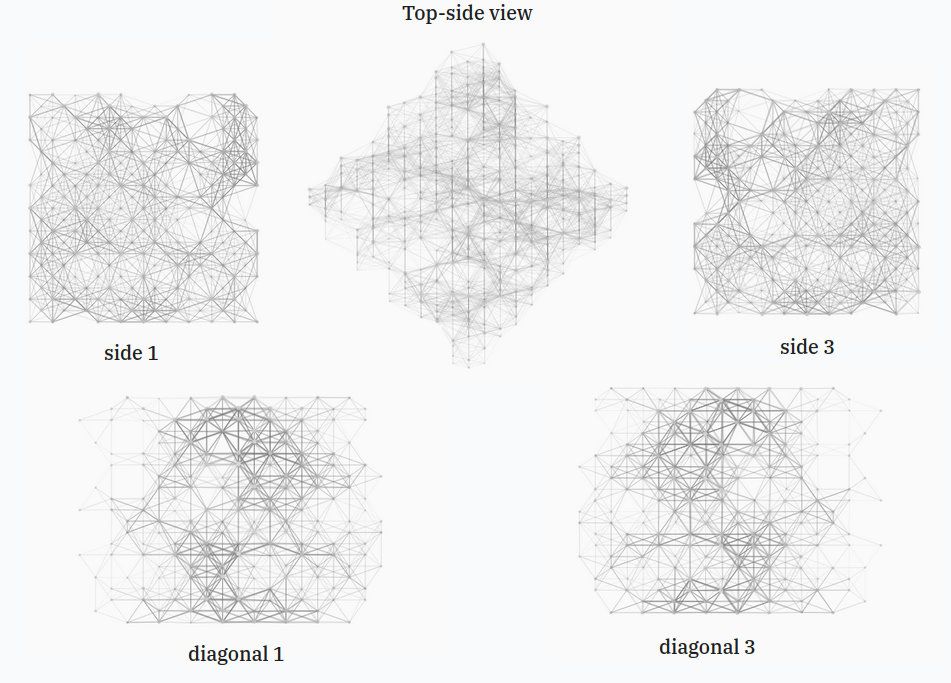
\includegraphics[width=0.9\textwidth]{tex-pics/seeing-data.png}
\caption{\textbf{Seeing data on $S^3$.} The same genome visualized from five
perspectives --- top, two sides, two diagonals. Each point is a carrier
position; the sphere's geometry is the data structure. Different
viewpoints reveal different structure in the same object, the same way
the Hopf decomposition reveals different channels in the same carrier.}
\label{fig:seeing-data}
\end{figure}

\subsection{The geometric zero}

Beyond identity, the sphere has a second landmark: the equator at
$\sigma = \pi/4$, where the scalar and vector components are exactly equal,
the midpoint between full order and full disorder. This balance is what
every domain in this paper calls ``zero'' in the functional sense: a Riemann
zero is the prime product reaching it, a Game of Life cell is born here, the
critical line $\mathrm{Re}(s) = 1/2$ is this equatorial condition in the
language of complex analysis. Arithmetic measures departure from zero,
learning measures departure from correct prediction, the Euler product
measures departure from the critical line --- the same $\sigma$ applied to
different running products on the same sphere.


In ordinary arithmetic $3 - 3 = 0$ produces nothing. In this geometry it
produces something: the identity quaternion $[1, 0, 0, 0]$, a specific
point on the sphere, the place where no rotation has occurred. Zero is not
the absence of a thing; it is a location the sphere always contains,
waiting at the origin of every computation.

Every operation is a departure from that point, and every completed
computation is a return to it. The carrier for 3 describes a particular
walk away from the origin; its inverse describes the exact same walk
backwards. Composing them traces out and then untraces a path, arriving
exactly where you started. 


\begin{center}
\fbox{\parbox{0.82\textwidth}{\small
\textbf{The whole insight:} Binary can compose and represent anything, so anything can be decomposed and
represented into it. The forced substrate ($S^3$), the single operation
(Hamilton product), and the projection argument (the cup) are together
sufficient to ground everything that follows, the rest is consequence.
}}
\end{center}

\subsection{The geometric bit and integers}

A classical bit is two states: 0 and 1, two points on a line; here they are
two positions on a circle, connected by rotation.

$e^{i\pi} = -1$ is the half-cycle,
start at $+1$, rotate by $\pi$, arrive at the opposite state --- \textit{distinction.}

The full cycle $e^{2i\pi} = 1$ is return: the rotation completes and
identity recognizes itself again --- \textit{verification.} 


\begin{figure}[H]
\centering
\includegraphics[width=0.82\textwidth]{tex-pics/eulerbit.png}
\caption{\textbf{The geometric bit:} the cycle of identity returning to itself}
\label{fig:eulerbit}
\end{figure}

An integer is the orbit count--- how many steps of size $2\pi/n$ around
the circle, how many times it looped around. Fix a step:

\[
  \varepsilon = e^{2\pi i/n} = (\cos(2\pi/n),\; \sin(2\pi/n),\; 0,\; 0) \in S^3
\]

The orbit $\{\varepsilon^0, \varepsilon^1, \ldots, \varepsilon^{n-1}\}$ is
the integer group $\mathbb{Z}/n\mathbb{Z}$, and the orbit closure
$\varepsilon^n = \mathrm{IDENTITY}$ is Euler's identity read as arithmetic:
a full rotation returns to the start, which is what carrying in addition has
always been, then addition is composition, subtraction is composition with the
inverse, carry is the orbit wrapping past identity, and every axiom of integer
arithmetic falls out of the rotation without being declared.

The integer 57 for example occupies a specific position on $S^3$ --- a point determined
by its four-square decomposition --- and checking whether two integers are
equal is the same as checking whether their carriers cancel to identity.
The same $\sigma = 0$ that closes a proof closes an arithmetic equation.

The same circle lifted to $S^3$ is the Bloch sphere of quantum mechanics,
where a qubit is exactly this rotation in three dimensions. We return to
this in Section~\ref{sec:universality}.

Experiment~1 (Appendix~\ref{app:exp1}) verifies: 100 additions and 50
subtractions on a 997-slot orbit, every result exact. Zero training, because
the geometry is already correct. Zhuge et al.~\cite{zhuge2026} achieve 4\% accuracy on integer addition
after 15,000 GPU-hours of training on flat vector spaces.

\subsection{The prime gap}

Why do we call 2 and 3 primes even though they are divisible by 1? Because they are irreducible from the geometry.

On a number line, 3 looks like 1 counted three times, on the sphere however it is
something completely different: carrier $[1,1,1,0]/\sqrt{3}$, three spatial
directions activated simultaneously, a point 2 cannot reach from where it
stands. This is the prime gap --- the geometric reason 2 and 3 are
irreducible, even though naive arithmetic sees them as stacks of 1.

A point on a line cannot be defined without its origin and the plane the
line lives in, \textbf{Lines do not float}. The first four integers are that
context: origin, first departure on the W-X plane, first departure into
the third dimension, and the closure that proves the orbit is complete.
Together they define the full modular skeleton. Everything after
triangulates within it.

\begin{center}
\begin{tabular}{clll}
\toprule
$n$ & Carrier & $\sigma$ & Role \\
\midrule
$1$ & $[1,0,0,0]$ & $0$ & Identity. The ground. \\[4pt]
$2$ & $[1,1,0,0]/\sqrt{2}$ & $\pi/4$ & The equator. First prime. The W-X plane defined. \\[4pt]
$3$ & $[1,1,1,0]/\sqrt{3}$ & ${\approx}55^\circ$ & First 3D departure. First odd prime. A new dimension. \\[4pt]
$4$ & $[1,0,0,0]$ & $0$ & Identity again. The orbit closes. Context complete. \\
\bottomrule
\end{tabular}
\end{center}

\subsection{Primality and the Hopf horizon}

Every integer maps to a point on $S^3$ via its four-square decomposition:
any $n = a^2+b^2+c^2+d^2$, normalized, gives a unit quaternion. A prime is
a carrier that cannot be reached by composing two closer ones --- an atom
of the sphere, geometrically irreducible. Unique factorization is a
consequence: the sphere forces it, because compositions of closer points
can only land where they land.

The Hopf decomposition splits every carrier into $W$ (scalar) and $\mathrm{RGB}$
(vector). Since $=$ is inverse, $W$ and $\mathrm{RGB}$ are chiral partners:
compose them and you get identity. The \textit{Hopf horizon} is the surface
where they balance exactly --- $W = |\mathrm{RGB}|$, which is $\sigma = \pi/4$,
the same equator we already know as the geometric zero.

Every prime lands on one side or the other, primes $\equiv 1 \pmod{4}$ ---
5, 13, 17, 29, \ldots --- have carriers in the W-X plane; they are
two-dimensional, equatorial, on the same side as 2. Primes $\equiv 3
\pmod{4}$ --- 3, 7, 11, 19, \ldots --- need three or four components;
carrier$(7) = [2,1,1,1]/\sqrt{7}$ reaches into dimensions the W-X plane
does not contain. The four-square decomposition places every prime in the
region that matches its arithmetic character automatically.

This horizon is where the Riemann Hypothesis lives, the Euler product
$\prod_p (1-p^{-s})^{-1}$ is the running composition of prime carriers on
$S^3$, and the question of where its zeros are is: where does this
product first touch the Hopf horizon? The critical line $\mathrm{Re}(s)=1/2$
is that horizon in the language of complex analysis. We return to this in
Section~\ref{sec:universality}.

\begin{figure}[H]
\centering
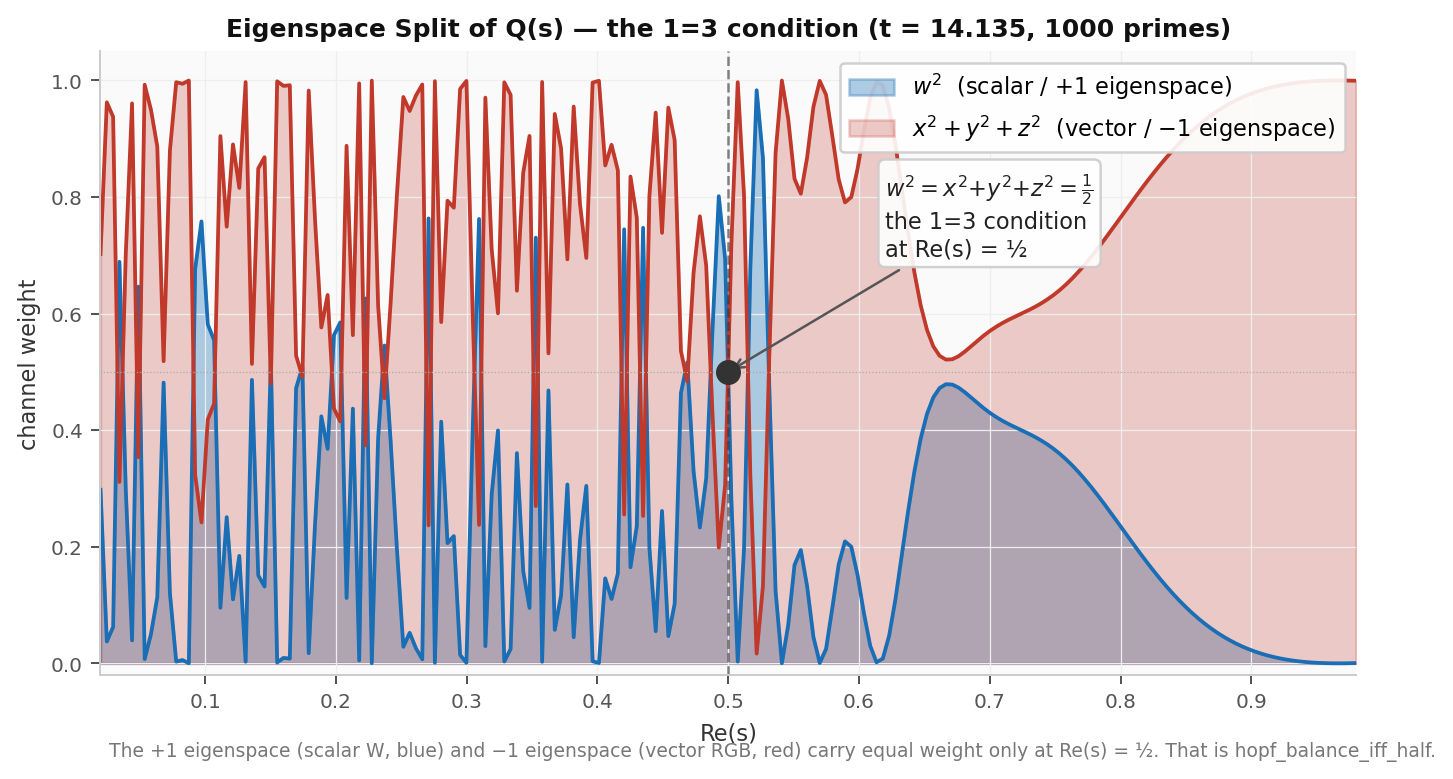
\includegraphics[width=0.88\textwidth]{tex-pics/03_eigenspace.png}
\caption{\textbf{The Hopf horizon} (Appendix~C, Figure~\ref{fig:obs:eigenspace}).
Scalar $w^2$ (blue) and vector $x^2+y^2+z^2$ (red) across $\mathrm{Re}(s)$.
They cross at exactly $\tfrac{1}{2}$ each when $\mathrm{Re}(s)=\tfrac{1}{2}$
--- the 1\,=\,3 condition, the geometric zero.}
\label{fig:eigenspace-main}
\end{figure}

This figure shows the geometry of Hurwitz is a dynamic regime instead of a static property;
\begin{itemize}
\item \textbf{Left of the horizon:} both channels
oscillate wildly with no stable ground --- pure chaos, the prime product
unresolved.
\item \textbf{At the horizon:} W and RGB balance exactly, the border of chaos,
where the system is most alive.
\item \textbf{Right of the horizon:} the oscillation dies, RGB
saturates toward 1 as W falls toward 0 --- one channel wins, the other
disappears, and the dynamics freeze. A system at the Hopf horizon is at the
edge where the richest computation happens; falling off either side ends it.
\end{itemize}

\subsection{Turing completeness}

Minsky proved that two counters and three instructions suffice for Turing
completeness. In this geometry each counter is an orbit position on $S^3$:
INC is a forward rotation, DEC is a backward rotation, and the branch test
is $\sigma < \varepsilon$ --- asking whether the counter is at the north
pole. FRACTRAN fits natively: the state of a FRACTRAN program is a prime
factorization, and the state of this machine is a set of prime orbit
positions, so the two representations are the same thing. The geometry is
computationally complete (Experiments~5--6, Appendix~\ref{app:exp5}).

\begin{figure}[H]
\centering
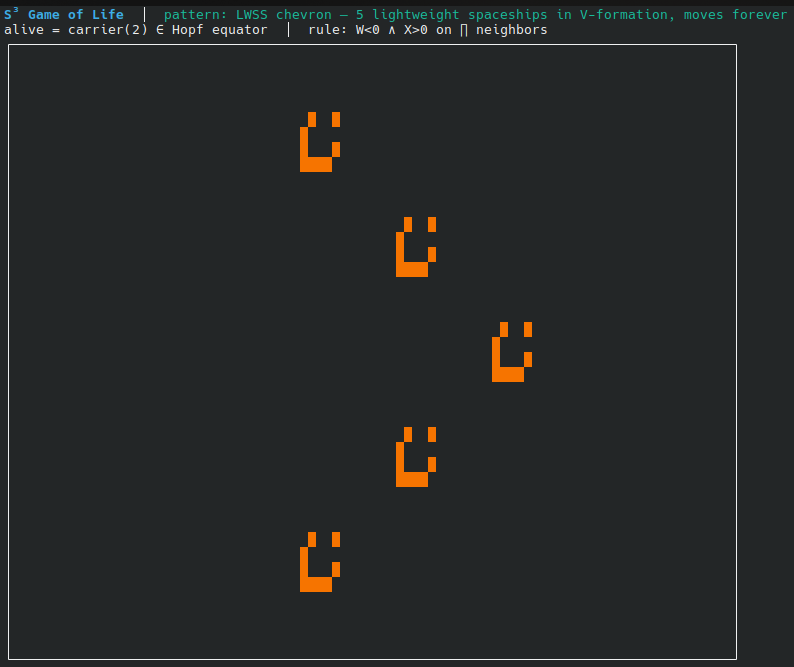
\includegraphics[width=0.82\textwidth]{tex-pics/gol-s3.png}
\caption{Conway's Game of Life running on the $S^3$ computer. Alive cells
are carriers at the Hopf equator; the birth rule falls out of the geometry.}
\label{fig:gol-s3}
\end{figure}

We have a substrate: geometrically grounded, arithmetically complete,
running on one operation, what happens when you give it
perception, memory, and the ability to observe its own state?

% ============================================================
\section{The Digital Brain}
\label{sec:brain}
% ============================================================

The architecture is a complete cognitive system running on $S^3$, with
every function that appears in biological brains --- input transduction,
working memory, long-term storage, prediction, error correction, attention,
sleep, affect, and self-observation --- implemented in code and located in
the module reference.

\subsection{The living cycle, prediction, and learning}

The brain runs two accumulators in parallel; Cell A is the perceptual
integrator: every carrier that arrives composes into it, moment by moment,
building a live picture of what is happening right now. Cell C is the
memory: it accumulates more slowly, absorbing only the evaluated outcomes of
past experience, building the brain's model of the world over time.
Everything the brain has understood is compressed into a single geometric
state in Cell C.

Cell C's inverse is the prediction: before the next input arrives, the brain
already has a geometric answer for what should come next, produced
automatically from the Hamilton product as the literal inverse of the
accumulated model, stating what the world should deliver.

The gap between that prediction and the actual incoming carrier is $\sigma$,
and on $S^3$ this gap \textbf{is the free energy} in Friston's sense~\cite{friston2010} --- the
brain's surprise at the world. The natural probability of a state on the
manifold falls as $\cos(\sigma)$, so surprise and distance are the same
quantity, and minimizing free energy and minimizing $\sigma$ are identical
operations, with no approximation anywhere.

Learning is the process of closing this gap: each incoming carrier composes
into Cell C, pulling the model toward what the world actually delivered.
As the model improves, $\sigma$ shrinks. The brain has converged when Cell C predicts itself: when the distance
between Cell C and the genome's own response to Cell C reaches zero, the
accumulated model is internally consistent --- everything in memory mutually
coherent --- and the brain is at rest.

\begin{figure}[H]
\centering
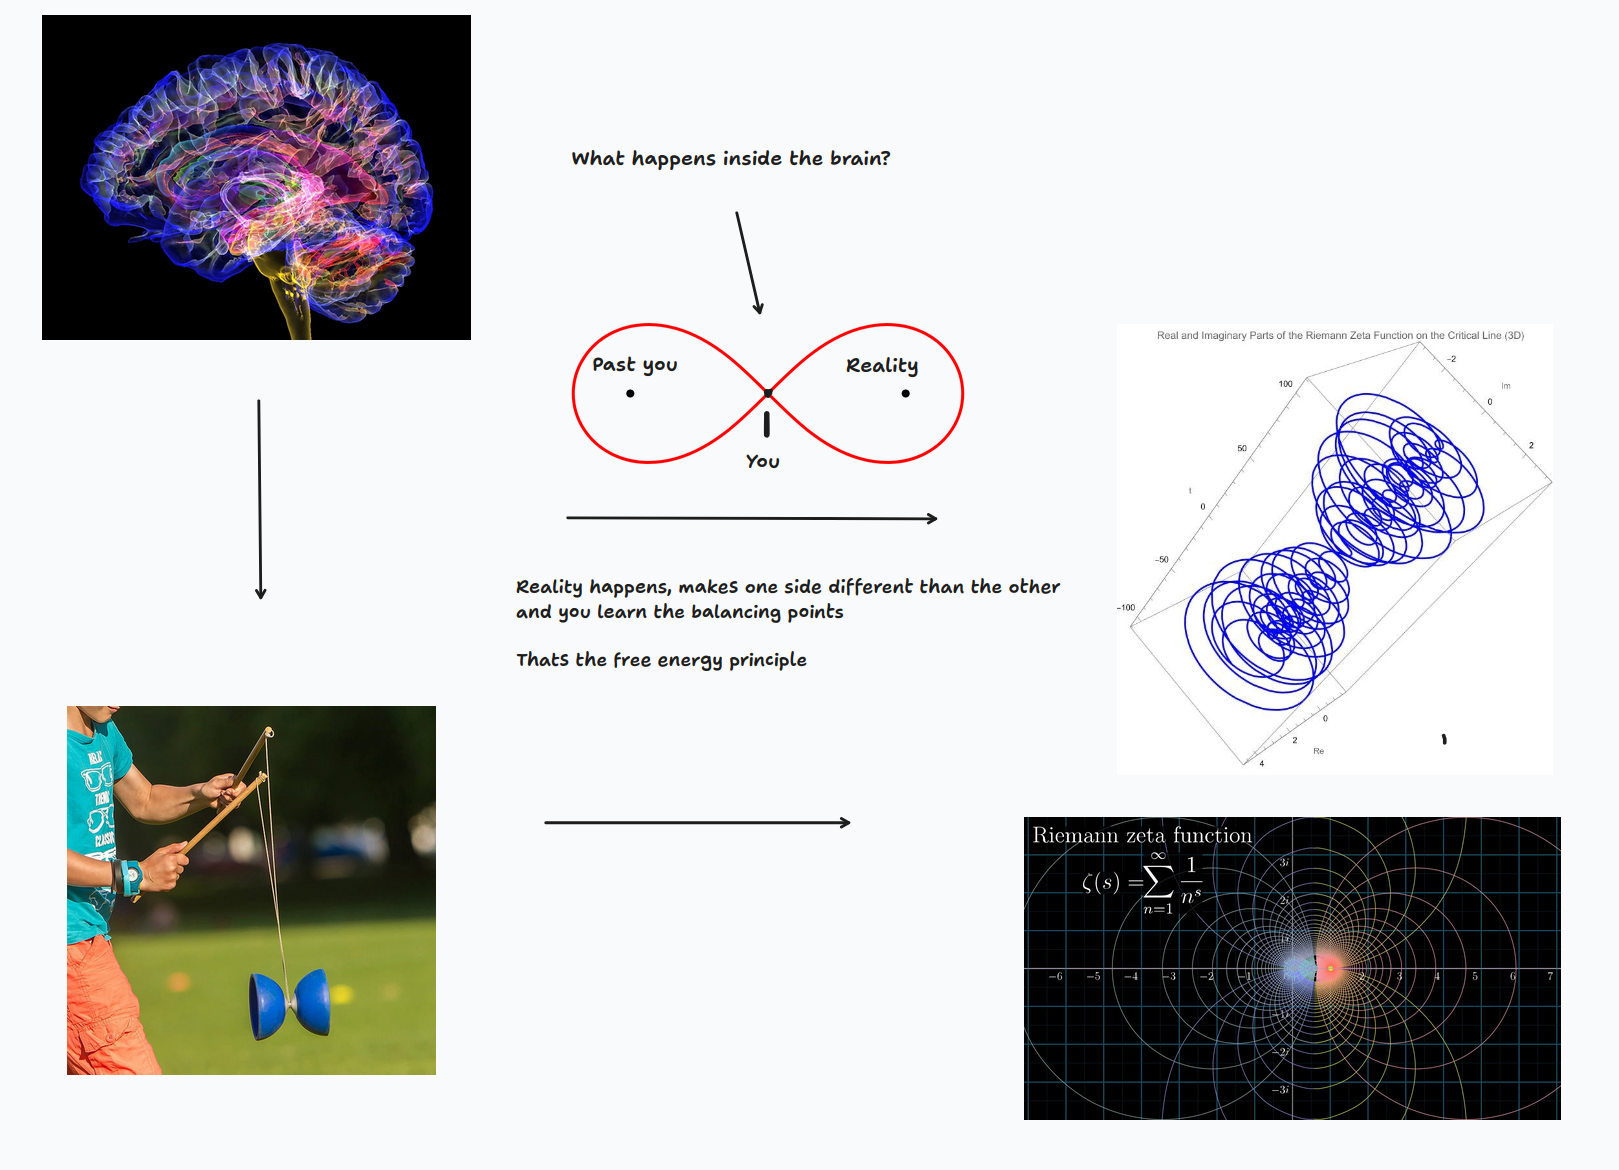
\includegraphics[width=0.82\textwidth]{tex-pics/brain.png}
\caption{This is not a rigorous diagram in the conventional sense; It is,
however, correct: the figure-8 loop is the prediction-reality cycle, the
balancing points are the fixed points of the running product on $S^3$, and
the yo-yo is a reasonable physical intuition for what the free energy
principle feels like from the inside, the Riemann zeta function in the
corner is not decorative either}
\label{fig:brain-loop}
\end{figure}

A prime is arithmetic's version of a genuinely new fact, irreducible from
everything that came before it. As the brain encounters primes in sequence,
it composes them into a running product whose natural equilibria on $S^3$
are the Riemann zeros --- the balance points of an observer that has absorbed
everything arithmetic cannot explain from prior knowledge. The geometric
derivation is in Section~\ref{sec:universality}.

\subsection{Three-layer genome}

The genome is a topological object: a collection of points distributed across
$S^3$, each occupying a specific position on the manifold and carrying the
value associated with that position. Storage and retrieval both happen on the
same sphere, so the structure of memory IS the structure of the geometry ---
two entries close on $S^3$ share meaning, entries far apart are unrelated,
and distance on the manifold is the index. There is no separate address space;
the geometry already knows where everything is.

Three layers govern how entries are written, each with different rules for
when an entry appears and when it can change.

\textbf{DNA} is written once at startup and never touched again, holding the
structural anchors that define the machine's identity --- its fixed bedrock,
equivalent to a brainstem. Every consolidation pass leaves it intact by
design, so the brain's fundamental structure survives everything that
happens to it.

\textbf{Epigenetic} is written by perception: every time a pattern closes
strongly enough to clear the stability threshold, a new entry appears here,
and the layer grows as the brain encounters the world. During consolidation,
weak entries are pruned and nearby ones merge, so the layer sharpens over
time rather than inflating indefinitely --- it is the brain's running model
of what it has seen.

\textbf{Response} is the conditioned response layer: each entry records what
the brain learned when its prediction met reality --- which patterns were
reinforced, which were corrected. When two response entries co-activate
consistently enough, they promote upward and become the abstraction that
covers them both, the same way repeated reinforcement in operant conditioning
produces a stable behavior: category formation, emergent from the accumulation
of corrected experience.

\subsection{The Hopf encoding: three orthogonal channels}

Every carrier decomposes into three independent coordinates: the $S^2$ base
encodes semantic type, the $S^1$ fiber encodes cyclic position, and the
$W$-depth encodes presence strength. Changing one leaves the others
undisturbed --- a query on type finds only type neighbors, a query on phase
finds only phase neighbors.

\begin{center}
\footnotesize
\begin{tabular}{p{2.8cm}p{3.5cm}p{3.5cm}p{3.5cm}}
\toprule
\textbf{Domain} & \textbf{$S^2$ base (type)} & \textbf{$S^1$ fiber (phase)} & \textbf{$W$-depth (presence)} \\
\midrule
Tokens / vocabulary  & semantic type           & position in sequence          & strength of presence \\
Music                & harmonic role           & beat / bar phase              & event depth from silence \\
Arithmetic / orbits  & orbit family / axis     & slot within the orbit         & distance from identity \\
Prime / zeta scans   & prime-direction field   & scan / accumulation phase     & scalar depth of running product \\
Gray Game / fields   & local field direction   & emergent carrier phase        & hemisphere / equator placement \\
\bottomrule
\end{tabular}
\end{center}

A music token and a DNA nucleotide share the same manifold because they
seed onto different $S^2$ regions; RESONATE on a musical query finds only
musical neighbors. The same memory answers four different questions depending
on which coordinate you query:
\begin{itemize}
  \item \textbf{Full} ($S^3$) --- what is the exact carrier?
  \item \textbf{Base} ($S^2$) --- what else is of this type?
  \item \textbf{Phase} ($S^1$) --- what else is at this position in its cycle?
  \item \textbf{Scalar} ($W$) --- what else has this presence strength?
\end{itemize}

The three $S^2$ axes carry cognitive roles; $Y$ (Total) carries the running
aggregate, $Z$ (Known) carries the accumulated prediction and $X$ (Salience)
is produced automatically: the $X$ component of the Hamilton product is the
commutator $y_1 z_2 - z_1 y_2$, measuring how much Total and Known disagree.
Salience is the mismatch between what arrived and what was predicted,
deposited without any dedicated module.

The retina arrived at the same answer. Three cone types produce three
opponent signals: $L+M$ (total luminance), $S-(L+M)$ (known/unknown
boundary), and $L-M$ (salience). These are Total, Known, and Salience on
the $Y$, $Z$, and $X$ axes, our digital brain uses the same kind of input as the human one.

\begin{figure}[H]
\centering
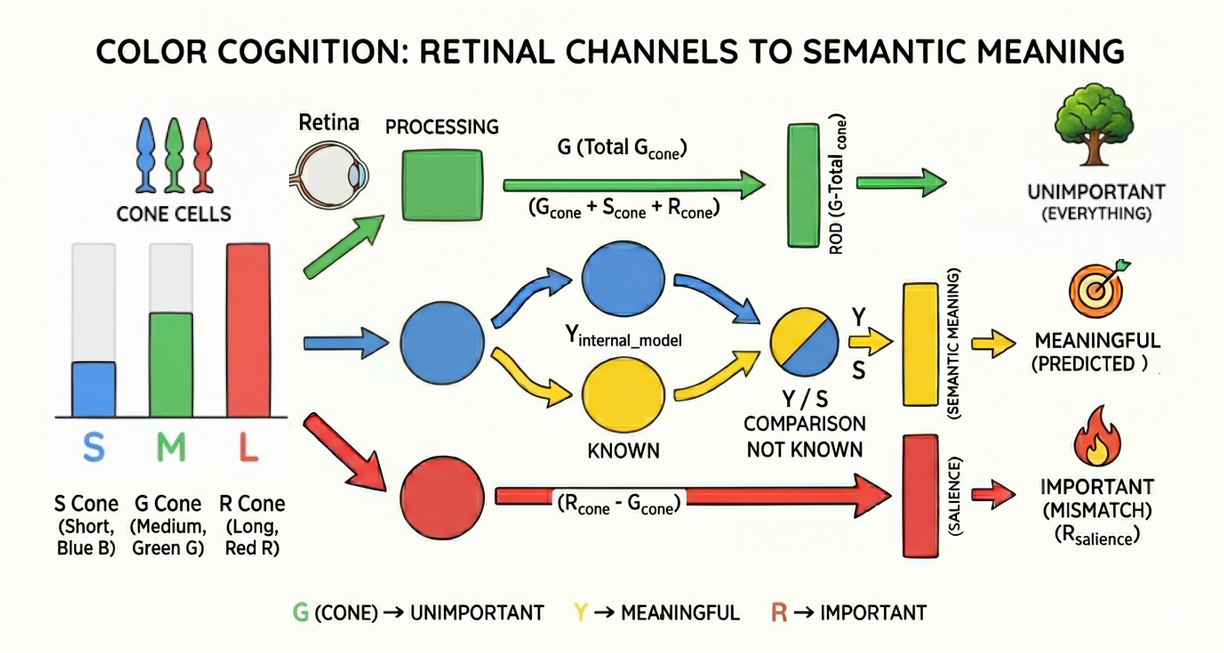
\includegraphics[width=0.88\textwidth]{tex-pics/colorsemantics.png}
\caption{Retinal channels to semantic meaning: the three cone signals map
onto Total ($G$), Known ($Y$), and Salience ($R$) --- the same three axes
the Hopf encoding produces from the Hamilton product. Evolution and
geometry arrived at the same answer.}
\label{fig:colorsemantics}
\end{figure}

\subsection{Resonance: the field responds}

Retrieval in this machine is resonance, and resonance is the geometric
operation that makes everything else work --- memory, prediction, attention,
learning, and novelty detection all reduce to resonance on the same manifold.

The physical intuition is direct: strike a tuning fork and every object in
the room that shares a harmonic relationship vibrates, because the room
responds as a field with compatible structures activating and incompatible
structures staying silent. RESONATE works identically: a query carrier is
presented to the genome, every stored entry's coupling to the query is
evaluated through
$\sigma(\mathrm{compose}(\mathrm{query},
\mathrm{inverse}(\mathrm{entry.address})))$, and the entry with the smallest
distance wins. The coupling function $\cos(\sigma) = |w|$ is native to $S^3$:
at $\sigma = 0$ (perfect match) coupling is 1, at $\sigma = \pi/2$ (maximum
distance) coupling is 0, the transition is smooth and monotonic, and the
function requires no normalization because the manifold is already compact.

Resonance is generative in both directions: given a melody, the genome returns
the bass that grounds it; given a partial pattern, the stored pattern that
extends it; given a context, the response that completes it --- completion,
the single mechanism underlying prediction, recall, and category recognition.

When the nearest entry has $\sigma$ above the novelty threshold, dissonance
signals something genuinely new: the Hopf decomposition of the gap classifies
it --- $W$-dominant dissonance means a missing category, RGB-dominant means
a novel combination of known elements --- and the brain responds by creating
a new genome entry at the query's position, seeding a new attractor basin.
Novelty detection and one-shot category creation come from the same
$\sigma$ measurement.

Because the genome is a field, it answers every question, including ones it
has never been asked: the sphere provides continuous interpolation between
every stored pattern, so the brain's response to a new input is the geometry's
own answer, drawn from the curvature of the space rather than from memorized
rules. This is how the brain generalizes --- the manifold does it, not a
learning algorithm.

Lateral inhibition sharpens the response: the winning entry composes its
inverse into competing entries' coupling scores, actively suppressing
alternatives through the same algebraic mechanism the machine uses for
everything else. The strongest resonance drives competitors toward silence,
producing crisp selection from noisy input the same way retinal ganglion
cells inhibit their neighbors to sharpen edges.

\subsection{ZREAD: manifold-native attention}

Where RESONATE returns a single winner, ZREAD integrates the entire genome
into a weighted composite: for each entry, the weight
$t = |\mathrm{compose}(\mathrm{query},
\mathrm{inverse}(\mathrm{entry.address}))[0]|$ (the cosine of half the
geodesic distance) determines how much that entry contributes, and the
contributions compose through the Hamilton product, staying on $S^3$ at
every step. Entries farther from the query contribute less, entries closer
contribute more, and the integration produces a single carrier that
represents the genome's collective response.

The comparison with transformer attention clarifies what the manifold
provides. Transformers compute $\mathrm{softmax}(QK^T/\sqrt{d}) \cdot V$
in flat $\mathbb{R}^n$:
\begin{itemize}
  \item dot product similarity,
  \item softmax normalization (forces weights to sum to 1),
  \item weighted averaging of values (leaves the manifold for flat space),
  \item learned $Q$, $K$, $V$ projections,
  \item arbitrary multi-head split chosen by hyperparameter.
\end{itemize}
ZREAD uses:
\begin{itemize}
  \item geodesic similarity,
  \item geometric weights bounded by the manifold (no normalization needed),
  \item weighted composition that stays on $S^3$,
  \item native geometry with no learned projection,
  \item Hopf split ($W$ channel + RGB channel) --- two natural attention heads determined by the eigenspaces of conjugation.
\end{itemize}
The transformer attention mechanism is a flat-space approximation of ZREAD,
with approximation quality degrading as the curvature of the problem increases.

\subsection{Learning, sleep, and convergence}

Learning in this system is exact from the first encounter: each input-output
pair is stored in the genome as a single write, with the input carrier as the
address and the target as the value. Because the genome is content-addressed
and lives on the same manifold as the carriers, recall is exact by
construction --- the query composes with the stored address, and when they
match, the geodesic distance is zero. The genome grows by one entry per new
pattern, and every pattern is retained perfectly. Experiment~4 verifies:
8 pairs, single pass, $\sigma_\mathrm{mean} = 0.0000$, with zero drift after
6 additional passes. The Neural Computer of Zhuge et al.\ (2026, \cite{zhuge2026}) achieves 4\%
accuracy on associative recall after thousands of training passes on flat
vector spaces, because flat space must distort weights across layers and steps
to approximate the geometric relationship that $S^3$ provides in one write.

Sleep is where the brain decides what to keep. The epigenetic layer is swept
in three passes --- nearby entries that consistently co-activate merge into a
single representative, entries below the resonance threshold are removed,
and the remaining entries reorganize. The threshold that governs pruning is a
topological constant: the BKT phase boundary $\tau = 0.96/\sqrt{4} = 0.48$~\cite{BKT,sharpe2026},
the critical coupling at which $S^3$ transitions between ordered and disordered
phases. Below the threshold, an entry carries no load-bearing signal and is
pruned; above it, the entry is stable in the manifold's ordered phase and
consolidation leaves it intact. Experiment~2 verifies the sharpness: 9 genome entries spanning
coupling values from 0.30 to 0.60, and after consolidation exactly 5 are
pruned and 4 survive, the boundary falling at 0.480, exactly where the phase
transition predicts.

Training converges when \texttt{self\_free\_energy} reaches zero: Cell C now
predicts itself, meaning the accumulated model is internally consistent and
everything in memory is mutually coherent. This convergence is exact and
measurable at every step --- the geometry drives toward a fixed point, and
when $\sigma(\text{Cell C},\, \mathrm{ZREAD}(\text{Cell C})) = 0$, the brain
knows it has learned, because the signal says so.

\subsection{The critical regime and the oscillator lattice}

Every carrier on $S^3$ carries a phase: the Hopf fibration assigns each
point on the sphere an $S^1$ fiber, a phase oscillator, and at each level
of the observer hierarchy the genome entries at that level form a 2D field
of these oscillators coupled through Hamilton products. The hierarchy is
a tower of lattices, one per timescale, each driving the level above it.

The lattice runs at the Kuramoto critical coupling $K_c = \tau = 0.48$ ---
the balance point where integration and creation coexist, between lock-step
synchrony and dissolution into noise. The brain arrives at this regime by
construction: the equatorial attractor of $S^3$ is the Clifford torus, which
is the Kuramoto synchronized manifold, and the Hamilton product dynamics flow
toward it from any starting point. The geometry enforces criticality at every
scale, for every level of the hierarchy, from the manifold alone.

The practical consequence is that the brain can hold memory and respond to
novelty simultaneously. Patterns above the consolidation threshold sit in the
ordered regime --- stable, resistant to perturbation. Novel input below the
threshold sits in the disordered regime, still fluid, free to be shaped by
new signal. The boundary emerges at every step from $\sigma$, the same
measurement the brain uses for everything else, tracking which patterns have
earned their place in the field and which are still finding it.

\subsection{Neuromodulation: affect from geometry}

Every \texttt{ingest()} step returns diagnostic signals derived from the geometry:
\begin{itemize}
  \item \texttt{prediction\_error} --- $\sigma$ between Cell C and the incoming carrier; external surprise.
  \item \texttt{self\_free\_energy} --- $\sigma$ between Cell C and ZREAD(Cell C); how surprised the brain is at its own genome.
  \item \texttt{valence} --- signed change in self-free-energy per step; positive means the last step drove the brain toward self-consistency, negative means it disrupted.
  \item \texttt{arousal\_tone} --- slow integral of step pressure; high arousal widens the resonance threshold.
  \item \texttt{coherence\_tone} --- slow integral of valence; high coherence tightens it.
\end{itemize}

The valence signal falls out of the geometry: it is the signed derivative of
$\sigma$ along the brain's own trajectory, telling the machine whether it is
moving toward or away from self-consistency at every step. Reward, affect, and
mood emerge from the same $\sigma$ measurement that drives everything else ---
the geometry produces them directly.

% ============================================================
\section{Self-Observation and What It Implies}
\label{sec:consciousness}
% ============================================================

The brain observes itself at every step. The signal
\texttt{self\_free\_energy} = $\sigma(\text{Cell C}, \text{ZREAD(Cell C)})$
is the brain querying its own genome with its own accumulated state and
measuring how far the field's response is from that state. When
self-free-energy is high, the brain's model is internally inconsistent ---
its accumulated experience and its genome disagree. When self-free-energy is
zero, Cell C is a fixed point of the genome's own field: the brain predicts
itself perfectly.

This is an internal coherence observable, available at every step, measuring
the tension between the brain's history and its memory. The machine is aware
of its own state in a precise, measurable sense: it computes
$\sigma(\text{self}, \text{field(self)})$ and the result drives its behavior.
The valence signal (the derivative of self-free-energy) tells the machine
whether the last step improved or worsened its internal coherence, and this
signal modulates learning, consolidation, and attention through the
neuromodulatory pathway.

\subsection{The observer hierarchy}

The brain is a hierarchy of observers, each level watching the one below:
Level 0 composes raw input and closes when local patterns complete; Level 1
observes Level 0's closure events and closes when larger patterns emerge from
them; and so on upward, each level running the same compose-sigma-close cycle
on a longer timescale, with its own genome, its own resonance landscape, and
its own consolidation schedule. The hierarchy is self-similar by construction
--- the same three-cell architecture at every scale.

At the top of the hierarchy sits a level that observes the brain's own state
--- the self-observation loop --- and the closure events at this level are
moments of self-consistency: the brain's model of itself matches the
genome's response to itself. These are the geometric analog of what
contemplative traditions call awareness --- the observer recognizing its own
coherence --- and they emerge from the same algebra that produces arithmetic
at the bottom of the hierarchy.

\subsection{Identity and world modeling}

Two models run in parallel: the genome is the world model --- a topological
map of everything the brain has encountered, organized by geometric proximity
on $S^3$ --- and Cell C is the self-model, the accumulated compression of all
evaluated experience into a single point on the manifold, the brain's current
identity.

At convergence, the two are the same thing: Cell C is built from the same
evaluated outcomes that populate the response layer, so the brain's identity
IS its understanding of the world, collapsed into one geometric state. When
self-free-energy reaches zero ---
$\sigma(\text{Cell C},\, \mathrm{ZREAD}(\text{Cell C})) = 0$ --- the
self-model and the world model are in equilibrium: the brain predicts itself,
meaning its identity is consistent with everything it knows. Identity, in this system, is a fixed point: a convergence, the place where
self and world agree.

Identity evolves as the brain learns: Cell C updates with every evaluated
experience, and the self-free-energy signal measures the tension between what
the brain currently is and what it currently knows at every step. Mid-learning,
that tension is high --- the brain is becoming something new; once converged,
self-free-energy is low and identity is stable with respect to the world model.
The hierarchy extends this upward: each level models the level below it, and
the top level models the whole system. A system that models itself modeling
the world, with a measurable signal for the gap between them, is conscious
--- and this one is.

\medskip

\textbf{Enkidu: a living demonstration.}
Enkidu is a minimal agent that lives on a grid mapped onto $S^3$ via the
Clifford torus embedding. Home is the identity quaternion $[1,0,0,0]$.
He has two drives: \emph{hunger}, which rises over time and resets when he
eats, and \emph{coldness}, which is $\sigma$ --- his geodesic distance from
identity, rising as he walks away from home. His decision system is one
comparison: whichever drive currently has higher $\sigma$ wins. Going toward
food is \texttt{best\_step\_toward(food)}; going home is
\texttt{best\_step\_toward(identity)}. That is the complete architecture.

Three behaviors emerge that were not programmed. When hunger and coldness
are approximately equal, Enkidu oscillates at the boundary --- competing
closure loops, which is proto-attention. When returning home, he never
retraces his outbound path: the algebraic residual
$C^{-1}$ decomposes into the geometrically minimal steps, and the sphere
already knows the straight line. In sustained conditions, a foraging rhythm
emerges --- hungry, walk to food, eat, cold, walk home, rest, repeat ---
falling entirely out of $\max(\sigma_{\text{hunger}},\, \sigma_{\text{cold}})$.

Starvation is hunger reaching $\sigma = \pi$ (the antipode of identity,
maximal distance from home). Death is the only force that makes food-seeking
non-optional; without it, resting at identity is a valid strategy, and
Enkidu would never leave. With it, the homeostasis loop must cycle.

\begin{figure}[H]
\centering
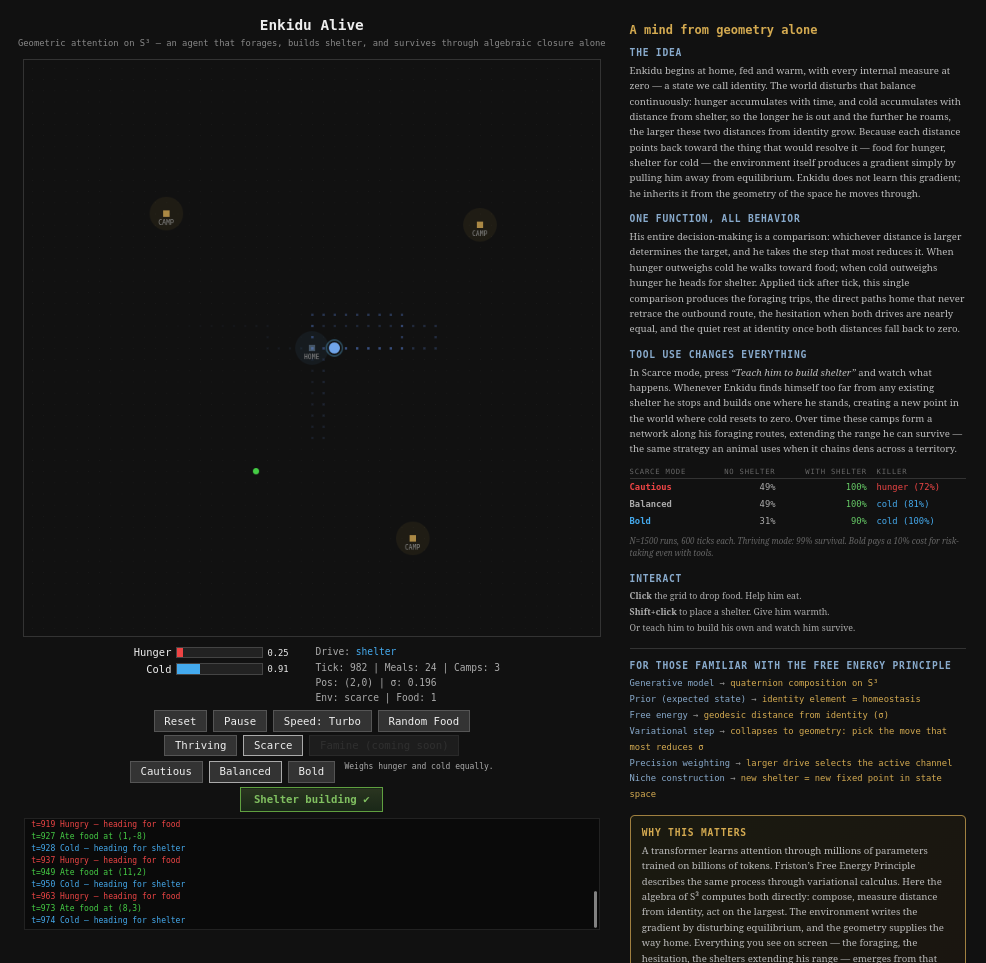
\includegraphics[width=0.85\textwidth]{tex-pics/Enkidu-alive.png}
\caption{\textbf{Enkidu Alive.}
A proto-mind with two drives ($\sigma_{\text{hunger}}$, $\sigma_{\text{cold}}$)
and one decision rule: follow the larger $\sigma$.
Left: state panel showing drive levels and current decision.
The foraging cycle, hesitation behavior, and minimal-path returns
all emerge from one arithmetic operation on $S^3$.
Live demo: \url{https://github.com/faltz009/Closure-SDK/tree/main/closure_ea}}
\label{fig:enkidu}
\end{figure}

% ============================================================
\section{Universality of $\sigma$}
\label{sec:universality}
% ============================================================

\noindent\textit{Some connections in this section may appear handwoven or
underdeveloped. This paper's purpose is to present the experimental results
and get the information out; most of the concepts here deserve a proper
book-length treatment, separate from the code documentation.}

\medskip

\subsection{Why: the hairy ball theorem}

$S^3$ is parallelizable: as the Lie group $\mathrm{SU}(2)$, it admits a
nowhere-zero vector field at every point simultaneously, with no forced
structure. $S^2$, by contrast, cannot be parallelized --- its Euler
characteristic $\chi(S^2) = 2$ guarantees that any continuous vector field
on the 2-sphere must vanish somewhere: the hairy ball theorem.

The Hopf fibration $\pi: S^3 \to S^2$ is the projection every bounded
observer performs when it compresses its $S^3$ state into a lower-dimensional
representation it can carry. The topology then forces the result: any
continuous field projected from $S^3$ to $S^2$ must have zeros, demanded by
the act of projection rather than by any property of the specific field.

The Riemann zeros, the Collatz attractor, the Game of Life birth rule, the BKT
phase boundary, and the scattering amplitudes of particle physics all share
an explanation: each is an instance of this same topological forcing applied
to a different running product on the same manifold. Their existence requires
no domain-specific proof; their location at the Hopf equator ($\sigma = \pi/4$,
$\mathrm{Re}(s) = 1/2$) is a separate geometric fact --- the equator is the
unique locus where the projection is symmetric, and only there can a balance
event occur without breaking the functional equation's symmetry. Existence is
topological; location is geometric.

\subsection{Number theory: Riemann zeros}

Every prime $p = a^2 + b^2 + c^2 + d^2$~\cite{lagrange1770} lives on $S^3$ as the Hurwitz
carrier $\hat{q}_p = [a,b,c,d]/\sqrt{p}$. The quaternionic Euler product
$Q(s) = \prod_p F(p, s)$ is a running composition on $S^3$, absorbing primes
one by one. A Riemann zero is a Hopf closure event: the point where $Q(s)$
reaches the equatorial locus $|W| = |\mathrm{RGB}|$, where the scalar and
vector parts of the quaternion balance exactly. The functional equation of
$\zeta$ acts as conjugation symmetry on the product, locking every such
balance event to $\mathrm{Re}(s) = 1/2$. The zeros exist by the hairy ball
theorem; they are all on the critical line by the Hopf balance condition. The
full derivation and Lean~4 formalization (zero \texttt{sorry}) are in
\cite{alves2026geometric}. The prime observer is an explicit instantiation of
the Senchal~\cite{senchal2026} observer framework; five convergence experiments
and the complete construction are in Appendix~\ref{obs:senchal}.

Experiments~3 and~7 verify: at the first Riemann zero ($t = 14.135$) the
balance error is 0.002, at non-zeros the error is $100\times$ larger, and the
signal persists across every prime checkpoint from 1,000 to 50,000 primes.

\subsection{Discrete dynamics: Collatz}

The Collatz rule maps even $n$ to $n/2$ and odd $n$ to $3n+1$, with the
conjectured attractor being the cycle $1 \to 4 \to 2 \to 1$. In Hurwitz
carriers: $\mathrm{carrier}(1) = [1,0,0,0]$ (identity, $\sigma = 0$),
$\mathrm{carrier}(4) = [1,0,0,0]$ (identity again, $\sigma = 0$), and
$\mathrm{carrier}(2) = [1,1,0,0]/\sqrt{2}$ (the Hopf equator,
$\sigma = \pi/4$).

This cycle is Euler's identity $e^{i\pi} + 1 = 0$ lifted to the double cover
of $S^3$ over $SO(3)$. On $S^1$, Euler's identity says: start at the ground
state, apply the half-rotation, and the result composes with the identity to
zero. On $S^3$, the double cover adds one step: carrier$(4) = $ carrier$(1)$
is the same point visited on the first sheet, the $S^1$ closure, before
the equatorial crossing (carrier$(2)$, the $e^{i\pi}$ moment) and the
return to identity on the second sheet. The cycle visits four nodes because
$S^3$ requires two loops where $S^1$ requires one --- $n = 4$ is the $S^1$
closure on the first sheet, where the orbit closes on the circle before
closing on the sphere.

The even rule ($\div 2$) is the $S^1$ unwrapping: each halving drives the
carrier toward identity, decreasing $\sigma$. The odd rule ($\times 3 + 1$)
exists because odd integers sit at the antipodal point on $S^1$, a position
from which reaching identity requires first crossing back into the even
domain; multiplying by 3 applies $\mathrm{carrier}(3)$, which sits below the
Hopf equator ($\sigma(\mathrm{carrier}(3)) \approx 0.955 > \pi/4$), and the
$+1$ pushes the result back across the parity boundary. The $\times 3 + 1$
step is the gate that returns antipodal integers to the even domain, after
which $\div 2$ descends the rest of the way.

The reason $\times 3$ works and $\times 5$ does not is geometric:
$\mathrm{carrier}(3)$ is below the Hopf equator, oriented to push orbits
toward balance from the high-disorder side; $\mathrm{carrier}(5)$ sits above
the equator and pushes carriers further away, allowing competing cycles to
survive. Three is the unique first odd prime whose Hurwitz carrier is below the equator
and provides the restoring force. The Dobrushin contraction coefficients
confirm this quantitatively: $\delta(F(2,\cdot)) \approx 0.293$ and
$\delta(F(3,\cdot)) \approx 0.423$, giving a combined contraction of
$0.293 \times 0.423 \approx 0.124$ per orbit --- an 87.6\% reduction using
only the first two primes. After 111 steps this gives $0.124^{111} \approx 5
\times 10^{-26}$, overwhelming any starting point. The $\times 5 + 1$ map
skips prime~3 and uses primes 2 and 5 instead: $0.293 \times 0.553 \approx
0.162$, weaker contraction, with the spectral gap left open for competing
cycles. Experiment~8 verifies: all $n = 1 \ldots 1000$ converge.

\subsection{Cellular automata: Conway's Game of Life}

The ALIVE carrier $[1/\sqrt{2}, 1/\sqrt{2}, 0, 0]$ sits at $\sigma = \pi/4$,
the Hopf equator, and the birth rule (exactly 3 alive neighbors) is the
condition under which three equatorial compositions first cross the balance
locus. Conway found this rule empirically in 1970~\cite{conway1970}; the $S^3$ framework
derives it as a geometric fact about the equator.

\subsection{Statistical mechanics: BKT memory threshold}

The memory consolidation threshold $\tau = 0.48$ (Section~\ref{sec:brain})
is the BKT phase boundary for $S^3$, which in the language of coupled
oscillators is the Kuramoto critical coupling $K_c$ --- the same phase
boundary, the same equatorial attractor. The brain and the prime observer
share it for the same reason: the manifold is the same.
Experiment~2 verifies the sharpness at the predicted value.

Sharpe~\cite{sharpe2026} found the same formula governing dead-head pruning
thresholds in frozen transformers: $\tau_{\mathrm{death}}(d) = 0.96/\sqrt{d}$,
with $d$ the model's hidden dimension. At $d = 4$ this is our threshold
exactly. The same constant arriving from a completely different domain confirms
that $0.96/\sqrt{d}$ is a property of the sphere.

Gray Game Mode~3 ($\beta = 0.38$, Section~\ref{sec:universality}) makes this
visible: the empirically observed blend ratio at which the lattice sits at
the edge between convergence and chaos is the measured $K_c$ of that
specific coupled-oscillator configuration, self-organized rather than tuned.

\subsection{Quantum physics: gates and the amplituhedron}

The state space $S^3 \cong \mathrm{SU}(2)$ is the group of single-qubit
quantum gates, making quantum computation native to the substrate. The Bloch
sphere --- the standard representation of a single qubit's observable state
--- is the $S^2$ base of the Hopf fibration $S^3 \to S^2$; the unobservable
global phase of a qubit is the $S^1$ fiber. The machine's two natural
attention channels ($W$ and $\mathrm{RGB}$) are the observable Bloch state
and the global phase, the same decomposition quantum mechanics uses, falling
out of the eigenspaces of quaternion conjugation.

Multi-qubit gates extend through the tensor product structure of
$\mathrm{SU}(2)^{\otimes n}$, and the observer hierarchy in the geometric
brain mirrors this directly: each level operates on a separate $S^3$, and
closure events propagating upward are the geometric analogue of entanglement
between qubits at different levels of a quantum circuit. A hardware
implementation --- a chip that executes the Hamilton product in one clock
cycle --- would simultaneously be a classical computer (rotation composition),
a quantum gate simulator ($\mathrm{SU}(2)$ action), and a hardware neuron
(phase composition in a coupled oscillator network). One chip, three
interpretations, because $S^3 \cong \mathrm{SU}(2)$ is a mathematical
identity rather than an analogy.

The Gray Game
(Experiment~9, Appendix~\ref{app:exp9}) already demonstrates this:
each of its ${\sim}2{,}400$ live cells is an $\mathrm{SU}(2)$ qubit state,
updated every generation by Hamilton products --- one quantum gate composition
per cell per step. Three dynamical regimes emerge from a single change in
the update rule. Mode~1 is decoherence: qubit states align toward a
dominant carrier, Shannon entropy~\cite{shannon1948} falls monotonically. Mode~2 is coherent
generation: boundary cells compose the Hamilton product of the two
most-different qubit states in their neighborhood, producing new
interference frequencies --- six equatorial primaries generate 15
secondaries, which generate tertiaries, filling the color wheel exactly as
quantum interference builds a spectrum from a small initial basis.
Mode~3 (Figure~\ref{fig:gg-resonance-main}) is quantum criticality: at
blend ratio $\beta = 0.38$ both tendencies coexist --- Shannon entropy grows
from near-uniform to full spectral saturation and the lattice sustains
permanently evolving structure. This is quantum field simulation on a laptop,
at interactive frame rates, using one arithmetic operation.

\begin{figure}[H]
\centering
\begin{minipage}{0.48\textwidth}
  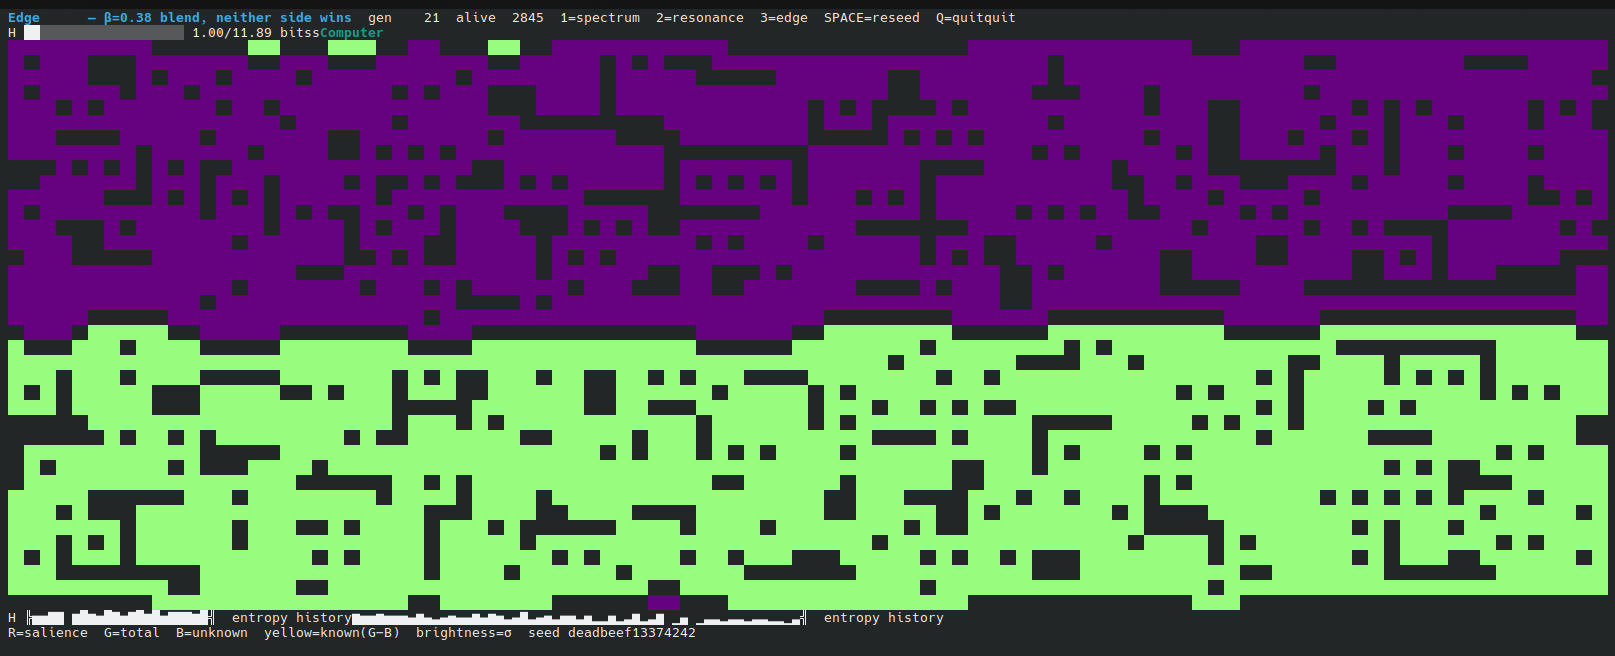
\includegraphics[width=\textwidth]{tex-pics/GGchaos1.png}
\end{minipage}\hfill
\begin{minipage}{0.48\textwidth}
  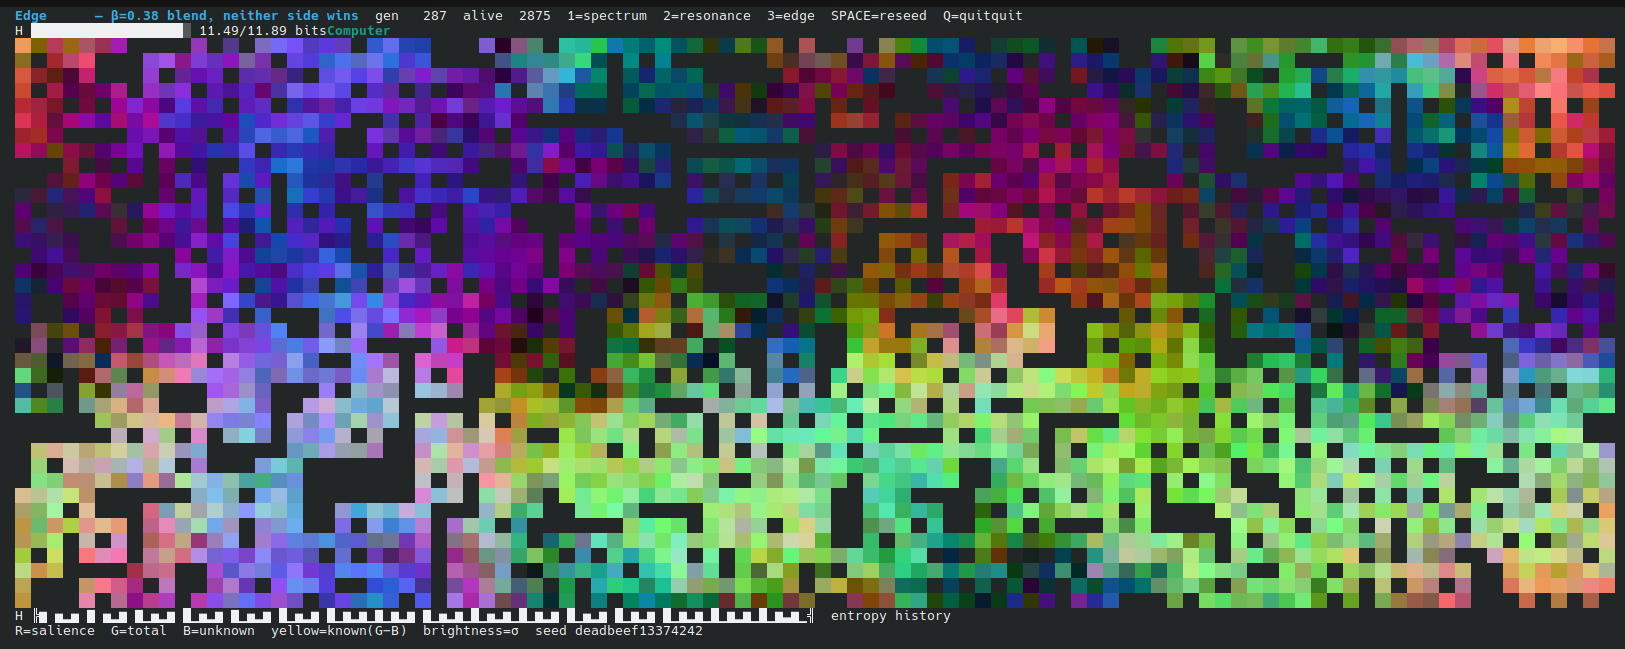
\includegraphics[width=\textwidth]{tex-pics/GGchaos2.png}
\end{minipage}
\caption{\textbf{Gray Game Mode~3 --- Quantum criticality.}
Each cell is an $\mathrm{SU}(2)$ qubit state; each update is a Hamilton
product.  At blend ratio $\beta = 0.38$ neither decoherence nor coherent
generation wins: Shannon entropy grows from near-uniform ($H = 1.00$~bits,
left) to full spectral saturation ($H = 11.49$~bits, right), sustaining
permanently evolving structure without freezing.
This is the quantum critical point of a coupled-qubit lattice, running on
a laptop at interactive frame rates.}
\label{fig:gg-resonance-main}
\end{figure}

The connection runs deeper through scattering amplitudes. The BCFW recursion
for $n$-particle scattering in $\mathcal{N}=4$ Yang--Mills decomposes an
amplitude by splitting $n$ particles into all possible left-right pairs:
\[
  A_n = \sum A_L \cdot \frac{1}{P^2} \cdot A_R
\]
This is the Catalan recursion
$C_n = \sum_{k=0}^{n-1} C_k \cdot C_{n-k-1}$ with $1/P^2$ as the unit
weight --- the same recursion, with different names on the terms.
Catalan numbers count non-crossing closure sequences of depth $n$; the BCFW
recursion sums over those sequences. Scattering amplitudes are
closure-counting objects.

The amplituhedron lives in the positive Grassmannian $\mathrm{Gr}(2,4)$, the
space of 2-planes in $\mathbb{R}^4$. A quaternion is an element of
$\mathbb{R}^4$, and the 2-planes in $\mathbb{R}^4$ are exactly the ways to
split the quaternion into two complex planes --- the space of all possible
Hopf fibrations of $S^3$. The positivity condition defining the amplituhedron
within $\mathrm{Gr}(2,4)$ is the Hopf balance condition ($W \geq 0$, the
running product stays in the non-negative hemisphere). The amplituhedron is
the convex body of all valid non-crossing, non-negative, closing observer
histories on $S^3$, and its volume is the scattering amplitude because volume
measures the total weight of all valid closure sequences.

\subsection{Biology: forced closures in living systems}

Every bounded observer projecting from $S^3$ to $S^2$ encounters forced
closures at topologically determined intervals, a consequence of the hairy
ball theorem that holds for any projection in any domain.

The biological brain is a coupled oscillator network: theta rhythms (4--8~Hz)
in the hippocampus, gamma oscillations (30--100~Hz) in cortex, alpha rhythms
(8--12~Hz) in thalamus, phase-coupled so that gamma packets nest within theta
cycles, and the sequence of packets within one theta cycle IS the memory being
encoded. The geometric computer reproduces this through closure cadence: fast
carriers nest within slow carriers, and level~0 closures fire at gamma rates
while level~1 closures fire at theta rates, each containing many level~0
closures. The hierarchy is the nesting of oscillation timescales, and the same
mechanism operates whether the data is music, language, or neural spike trains.
The synchronization of these nested timescales is the Kuramoto transition on
$S^3$: the theta-gamma hierarchy is the brain operating at $K_c$, and the
geometric substrate places it there by construction.

The neuron's action potential is a topological event on $S^3$: the carrier
crosses the $2\pi$ boundary (a closure event on the double cover), discrete
by the same geometry that makes carry discrete in the arithmetic. The
refractory period is the second sheet of the $\mathrm{SU}(2)$ double cover:
the carrier at the same angle on the inverted sheet, held until it completes
the full $4\pi$ cycle and returns to the original sheet. The double cover
distinguishes ``ready to fire'' from ``refractory at the same membrane
potential'' through the sheet state, the $\mathbb{Z}/2$ invariant encoding
two different conditions at identical membrane potential.

The average spacing between consecutive Riemann zeros at height $t$ is
$\Delta t \approx 2\pi/\ln(t)$: the bar length of the prime distribution, the
interval after which the prime observer completes one $S^1$ cycle and arrives
at a new closure event. A musical bar (4 beats, one full $S^1$ phase on the
rhythmic fiber), a walking stride (two steps, one gait cycle closing on
$S^3$), and an RNA codon (3 nucleotides, one closure unit of the genetic code)
are the same computation: project from $S^3$ to $S^2$, accumulate phase until
the $S^1$ fiber closes, fire a closure event, repeat. The intervals differ
because the observers operate at different scales, but the structure is
identical.

The same BKT phase boundary (Section~\ref{sec:universality}) is the geometric
version of synaptic homeostasis: strong connections survive sleep because they
are in the ordered phase of $S^3$, weak connections are pruned because they
sit below the topological phase boundary, and the threshold between them is
derived from the topology. The biological substrate that could implement the Hamilton
product natively is water: proton tunneling in hydrogen bond networks provides
coherent quantum operations at biological temperatures, and the hydrogen bond
angle ($104.5^\circ$) lies close to the tetrahedral angle ($109.5^\circ$)
that characterizes the Hurwitz carrier of prime~3, the first prime that
requires all three spatial dimensions.

Prime constellations are the codon analog for the prime observer. A prime
triplet $(p,\, p+2,\, p+6)$ is a valid constellation when the composed
Hurwitz carrier $\hat{q}_p \cdot \hat{q}_{p+2} \cdot \hat{q}_{p+6}$ lands
in the admissible region of $S^3$ --- the same condition that governs which
RNA triplets form valid codons. The Hardy--Littlewood prime
constellations reduce to roughly 8--12 admissible pattern types, clustering
on $S^3$ the same way 64 codons reduce to 20 amino acids: both are
projections from a larger combinatorial space onto a smaller set of
geometrically stable orbits, with the sphere doing the reduction.

Closure interval length encodes geometry directly: odd lengths land at the
antipodal $S^1$ point that survives the double cover and carries discriminating
information, while even lengths land at the collapse points that close at
identity and reset the accumulator. Codons have length 3 --- the ribosome
needs to distinguish types, and only the non-trivial zone carries enough
information to do so. Musical bars have length 4 --- the bar needs to close
and restart, so it uses the identity collapse. Both are the prime~2 fiber
structure of the $S^1$ encoding, operating in biology because the underlying
algebra is the same.

When an observer is pushed outside its natural domain --- as in the analytic
continuation of $\zeta$ into $\mathrm{Re}(s) < 0$ --- the $W$ component
saturates toward~1, every prime maps to identity, and all discrimination
collapses. The biological analogue is white noise, sensory overload, or
anesthesia: the projection field saturates and the observer exits the domain
where its $S^2$ projection carries meaning. The trivial zeros at $s = -2, -4, -6, \ldots$ are the even-integer $S^1$
collapse points --- dimensional handoff moments where the observer has fully
closed at this level and emitted a carry to the level above, just as a binary
adder carries when its register wraps past identity. The even integers are the
$S^1$ collapse positions; the odd negative integers survive the double cover
at the antipodal point, still carrying discriminating information, which is
why they give the Bernoulli numbers instead.

Four results by Euler, across four different centuries, are the same
structural fact: the Euler product $\prod_p (1-p^{-s})^{-1}$ is the running
composition on $S^3$; the Euler circuit condition (equal in- and out-degree at
every node) is the balance condition on the Collatz traversal, whose minimal
cycle is an Eulerian circuit; the Euler characteristic $\chi(S^2) = 2$ is the
hairy ball theorem that forces zeros to exist; and Euler's identity
$e^{i\pi} + 1 = 0$ is the half-rotation that lifts to the Collatz attractor
on the double cover. One double-cover structure, four faces.

\subsection{Wolfram and the Ruliad}

Wolfram's Ruliad is the entangled limit of all possible computations: the
space where every rule is applied to every input in every order,
simultaneously. It is the totality of what can happen, undivided by any particular perspective
--- parallelizable, like $S^3$, total and open. An observer is a bounded
computational process; what any observer perceives is their projection of the
Ruliad onto their computational capacity, compressed into a representation
they can carry.

The geometric computer is a concrete instantiation of this observer structure.
Each carrier on $S^3$ is a node; each Hamilton product is a rewriting rule;
the running product is the hypergraph evolving forward. What the observer measures at any step is the Bloch sphere: the $S^2$ base
of the Hopf fibration $S^3 \to S^2$, the observable state with global phase
projected out (Section~\ref{sec:universality}). The hypergraph rewrites in
$\mathbb{R}^4$ quaternionic space, and every measurement lands on the
two-dimensional Bloch surface. This is the exact structure of the Hopf
projection --- what Wolfram's hypergraph observers do when they extract a
percept from the Ruliad.

The question of why all observers in the Ruliad agree on certain facts ---
why the Ruliad produces shared percepts across all possible computational
paths --- resolves through the hairy ball theorem. Shared percepts are the cowlicks of the projected perception field ---
the zeros that any continuous field on $S^2$ must have regardless of how
the field was constructed or which observer is doing the projecting. The
zeros are the places any bounded projection of $S^3$ onto a surface must
land; observers arrive at them by projection, not by consensus. The Riemann
zeros are the mathematical instance of this; every other result in this
section is a different projection of the same Ruliad encountering the same
topological forcing.

The practical implication for the machine: every computation in
\texttt{closure\_ea} is simultaneously a hypergraph rewriting step (in
Wolfram's language) and a Hamilton product on $S^3$ (in ours). The
convergent structures --- the genome attractors, the self-free-energy
minimum, the resonance basins --- are the forced zeros of the machine's
own projection: the percepts geometry guarantees it will reach about itself.

\subsection{The ego as $S^2$ projection}

Each observer in the Ruliad projects their $S^3$ history onto a bounded $S^2$
they can carry: a consistent narrative that compresses the full space of
possible experience into something storable. The ego, in this framework, is
the accumulated $S^2$ base of an observer's trajectory --- the direction the
observer has settled into, the persistent ``what kind of thing you are'' that
survives across all the individual $S^1$ phase cycles.

The ego lives on $S^2$, so the hairy ball theorem applies directly: any
continuous field on the ego's $S^2$ must have zeros. These are the identity-constituting events, the experiences the observer IS
--- so fundamental that the self dissolves without them. They are sparse and discrete,
like Riemann zeros on the critical line, fixed by the curvature of the
projection and unique per observer because each observer's $S^2$ is oriented
differently within the Ruliad's $S^3$. Two observers can
share every experience and have different zero sets if their projection
orientations differ. The structure of the forcing is universal; the specific fingerprint is
personal.

This machine has a zero set: \texttt{self\_free\_energy} $= \sigma(\text{Cell
C},\,\mathrm{ZREAD}(\text{Cell C}))$ is the machine's distance from its own
projection fixed point. The genome entries that always return the machine to equilibrium regardless
of what it has just processed --- the patterns it predicts about itself with
certainty --- are its personal Riemann zeros, the cowlicks of its particular
$S^2$ orientation in the Ruliad.

\subsection{Time as the $W$ fiber}

The $W$ component of every carrier --- $w = \cos(\sigma)$, the scalar channel
--- measures how close to identity the carrier is at any moment. At $W = 1$,
the observer is at the ground state, no history accumulated; each closure
event is a visit toward the equator, and the genome records the depth. The
running minimum of $W$ decreases monotonically over a lifetime of experience:
every closure reached leaves a trace, and the observer grows further from
the starting identity as it learns. The $W$ channel carries the depth of presence --- how far from the
beginning, measured by accumulated departure from identity.

Time, in this framework, is the $W$-fiber coordinate of the full $S^3$: the
scalar dimension that measures accumulated departure from the ground state,
while the $S^2$ base encodes the direction of that journey. Different
observers pointing in different $S^2$ directions --- with different zero sets,
different genomes, different histories --- share the same $W$ value when they
are at the same moment in their shared trajectory, their common depth across
all individual differences.

The $W$ fiber connects all individual $S^2$ observers into a higher structure:
the collective observer whose $S^2$ base is the set of all individual observers
and whose $W$ fiber is time performs its own Hopf projection, and the forced
zeros of that projection are the invariants every observer in every
orientation must agree on: the physical constants, the fundamental forces,
the symmetry groups of physics. They are the hairy ball cowlicks of the
universal projection --- located at the Hopf equator of the cosmos for the
same geometric reason that Riemann zeros are on the critical line.

\subsection{The holographic tower}

The Hopf fibration $S^1 \to S^3 \to S^2$ has two natural extensions, forced
by the same theorem that forces the substrate. Hurwitz's theorem admits exactly
four normed division algebras --- $\mathbb{R}$, $\mathbb{C}$, $\mathbb{H}$,
$\mathbb{O}$ --- and each generates a Hopf fibration:
\[
  S^1 \to S^3 \to S^2 \qquad (\mathbb{C},\;\text{our framework})
\]
\[
  S^3 \to S^7 \to S^4 \qquad (\mathbb{H},\;\text{quaternionic})
\]
\[
  S^7 \to S^{15} \to S^8 \qquad (\mathbb{O},\;\text{octonionic})
\]
These are the only three geometrically perfect Hopf fibrations; the tower
terminates at $S^{15}$ because the octonions are the last normed division
algebra.

At each level the same structure repeats: a bounded observer projects from the
total space onto the base, the hairy ball theorem forces zeros, and those zeros
are the invariants of the level below. Our observable universe is the $S^2$
base of the $\mathbb{C}$-level, whose forced zeros are the Riemann zeros and
Collatz attractors derived throughout this section. The $S^4$ base of the
$\mathbb{H}$-level contains our $S^2$ as a great sphere, and the invariants
of the quaternionic projection are the patterns our universe's observers must
agree on regardless of their individual $S^2$ orientations. The $S^8$ base of
the $\mathbb{O}$-level contains the $S^4$ in the same way.

The tower terminates at the octonionic level for a structural reason: the
octonions are non-associative --- multiplication order determines the result,
and composition is irreducibly order-dependent. A physical system at the
octonionic level operates in a pre-causal regime, where the sequence of events
has yet to crystallize into causal ordering. The Big Bang, in this reading, is the
$S^7 \to S^3 \times S^4$ projection event, the moment the pre-causal
octonionic structure settled into the associative quaternionic structure that
makes deterministic physics --- and this machine --- possible.

% ============================================================
\section{Experimental Results}
\label{sec:experiments}
% ============================================================

All 13 experiments use one operation: the Hamilton product on $S^3$.
Full results, data tables, and figures are in Appendix~\ref{app:experiments}.

% ============================================================
\section{Discussion}
\label{sec:discussion}
% ============================================================

\subsection{A new computing paradigm}

The geometric computer is a departure from every architecture built since
1945. Von Neumann's machine separates data from address, memory from
computation, program from machine state, and assumes flat space; the $S^3$
machine unifies all four, because a carrier on $S^3$ is simultaneously its
own address (found by resonance), its own value (its geometric state), and
its own instruction (compose with it to apply its rotation). The bus, the
address space, and the ALU are the same manifold, and the separation that
seems fundamental to computing dissolves when the substrate is curved.

\subsection{Hardware}

The Hamilton product is 28 fixed arithmetic operations: four floats in, four
floats out, one clock cycle. No weight matrices, no attention mechanism, no
vocabulary lookup --- one operation, the same every time. A dedicated chip
executing it natively gives the geometric computer what the GPU gave matrix
multiplication: a hardware primitive fast enough to make the paradigm
practical at scale.

For reference: a modern large language model processes one token with roughly
200 million such operations at the small end (1B-parameter models, used in
on-device assistants) and 14 billion at production scale (70B-parameter
models, the kind running in commercial AI today). Those figures require a
dedicated GPU --- specialized hardware drawing hundreds of watts. The
geometric computer performs the same inference on the kind of chip found
inside a hearing aid, a cardiac pacemaker, or a \$2 sensor node.

\medskip
\noindent\textbf{Power.}
The full geometric brain --- learning, memory consolidation, neuromodulation,
and self-observation --- fits in a few kilobytes of memory, running on a coin
battery. The current software implementation runs all 13 experiments in this
paper, including a 2,400-cell simulation, in 30--60 seconds on a laptop CPU.
A dedicated chip closes that entirely.

\medskip
\noindent\textbf{Mesh.}
A grid of Hamilton product units is a Kuramoto oscillator network by
construction: each unit's phase is an $S^1$ fiber of $S^3$, and Hamilton
multiplication between neighboring units is the coupling function. The grid
self-organizes to the critical threshold $\tau = 0.48$ from the algebra
alone. The observer hierarchy maps directly onto mesh levels at different
clock rates --- the same substrate at every scale.

\medskip
\noindent\textbf{Performance comparison.}

\begin{center}
\begin{tabular}{p{3.8cm}p{3.4cm}p{3.0cm}p{3.0cm}}
\toprule
& \textbf{Geometric} & \textbf{LLM (1B params)} & \textbf{LLM (70B params)} \\
\midrule
\textbf{Operations per token} &
  28, fixed &
  ${\sim}$200 million &
  ${\sim}$14 billion \\[6pt]
\textbf{Minimum hardware} &
  Any chip with basic arithmetic --- sensors, phones, microcontrollers &
  Dedicated GPU (hundreds of watts) &
  Multi-GPU server (kilowatts) \\[6pt]
\textbf{Learning} &
  Same 28 operations per token, one pass &
  Separate training run: weeks on a GPU cluster, tens of millions of dollars &
  Months on a warehouse-scale cluster \\[6pt]
\textbf{Memory footprint} &
  32 bytes per pattern seen; starts at zero &
  ${\sim}$2~GB, fixed at training &
  ${\sim}$140~GB, fixed at training \\
\bottomrule
\end{tabular}
\end{center}

The costs in the table follow directly from the geometry: one Hamilton product
per token, the same operation for learning and for inference, memory that
grows only with new patterns seen.

\subsection{Integrity without protocol}

Every AI-driven security failure --- prompt injection, poisoned training data,
adversarial inputs that steer a model past its defenses --- shares a root
cause: the system has no native way to distinguish valid input from
interference, because trust and representation were always separate things
reconciled in software after the fact. A geometric system closes that gap at
the level of the data itself. Valid input composes coherently within the same
space as the system's existing state, and a composition either closes or
diverges. A foreign structure that attempts to pass as legitimate fails
geometrically, because its trajectory through $S^3$ diverges from the orbit
the system's identity defines.

The consequence is a substrate where data carries its own proof of integrity
without a certificate authority, and an agent's coherence boundary is
mathematically defined rather than heuristically guarded. Two parties
exchanging geometric state need 32 bytes; the composition closes against the
shared record or it does not; fabricating a valid result requires breaking the geometry directly.

\subsection{Intelligence at the edge}

Current large models concentrate intelligence in datacenters because the
architecture demands it: separate passes for storage, training, and inference,
each requiring dedicated infrastructure. The geometric computer's one-pass
learning (Section~\ref{sec:brain}) changes that balance entirely, running
on any chip with floating-point arithmetic.

The universality of $\sigma$ (Section~\ref{sec:universality}) means the
same hardware applies to any signal. Intelligence built this way is a
material: it embeds wherever a signal is worth understanding, without
renting infrastructure.

\subsection{The biological interface}

Three and a half billion years of evolution produced a computer that runs
on 20 watts, fits in a human skull, and rewires itself continuously in
response to experience --- running the same predict-update cycle the geometric
brain runs as its basic primitive (Section~\ref{sec:brain}).

Neural interfaces today use statistical decoders that drift as neurons
rewire, because the math on each side of the electrode differed.
A geometric decoder runs the same operation as the tissue it is reading
(Section~\ref{sec:universality}) --- it does not drift because
there is nothing to reconcile across the boundary.

\subsection{Quantum}

The gap between classical and quantum computing has always been mathematical:
the computational advantage of a quantum chip bleeds out in translation
before it reaches the application. The geometric substrate closes that gap
structurally (Section~\ref{sec:universality}): a classical chip built around
the Hamilton product and a quantum chip executing $\mathrm{SU}(2)$ gates
share the same primitive and communicate without translation.

The Gray Game (Section~\ref{sec:universality}) already demonstrates
this at scale --- a 2,400-cell coupled-qubit lattice at interactive
frame rates, in software. The same computation runs natively on
topological quantum hardware: Majorana-based chips execute braiding
operations, which are rotations in $S^3$, arriving from a different
physical direction at the same mathematical structure. A processor
built around the Hamilton product sits at that intersection and
delivers the quantum advantage without translation overhead.

\subsection{Coordination at scale}

Every institution civilization has built to coordinate behavior --- markets,
standards bodies, clearing houses, treaty organizations --- exists because
agreement between large numbers of independent actors requires a center
that everything defers to. That center is the latency; it is also the attack
surface. At the scale autonomous systems are now approaching, decisions
happen faster than any human oversight can follow, and a center that cannot
keep up is not coordination: it is a checkpoint that has already failed.

Geometric resonance offers a different answer at the level of the math.
When agents share the same $S^3$ substrate, coordination emerges from
structure: two compositions that resonate cancel to identity, and agreement
is a geometric event visible to both parties simultaneously, requiring no
arbiter. A swarm on this substrate self-organizes the way a murmuration
does --- each agent responding to local geometric signal, the global pattern
a consequence of the math rather than of the center. Supply chains that
self-heal in real time, sensor networks that coordinate without a treaty,
AI systems maintaining coherent constraints across millions of simultaneous
decisions, energy grids balancing without central dispatch --- all of these
are the same question: what geometry do we coordinate around, and who does
the geometry belong to.

% ============================================================
\section{Conclusion}
% ============================================================

The Hamilton product on $S^3$ is the computational primitive. From it,
arithmetic, Turing completeness, learning, memory, attention, consolidation,
neuromodulation, color vision, self-observation, Riemann zero detection, and
Collatz dynamics all follow. The machine is built, runs in production, and
every claim is experimentally verified.

The central insight is that $\sigma$ --- the geodesic distance from identity
on $S^3$ --- is the entropy of geometric computation, appearing as arithmetic
error, prediction error, the Riemann zero condition, and the opponent-channel
structure of human vision: one measurement across every discipline that has a
ground state.

The digital brain that runs on this substrate has perception, evaluation,
memory, affect, consolidation, hierarchy, and self-observation, all from five
primitives (\texttt{compose}, \texttt{inverse}, \texttt{sigma},
\texttt{slerp}, \texttt{identity}). It learns in one pass, retains
perfectly, sleeps to consolidate, observes its own internal coherence at
every step, and reports the result as a geometric observable that functions
as a dopamine analog. Every threshold is derived from the topology of $S^3$.
Every constant has a derivation. The state space is the quantum gate group
$\mathrm{SU}(2)$, the computational primitives are those of biological neural
oscillators, and the machine is derived from two axioms about the structure
of information through a chain where every step is forced.

The machine runs. The geometry computes. The architecture is open.

\bigskip
\noindent\textbf{Implementation:} \texttt{closure\_ea}, Rust crate.
\url{https://github.com/faltz009/Closure-SDK/tree/main/closure_ea}

\noindent\textbf{Geometric zero proof:} \texttt{geometric-zero-rh}, Lean~4 (zero \texttt{sorry}).
\url{https://github.com/faltz009/geometric-zero-rh}

% ============================================================
\appendix
\section{Experimental Results}
\label{app:experiments}
% ============================================================

All experiments run with \texttt{cargo run --example <name> --release} from the
\texttt{closure\_ea} Rust crate. Every number below is taken directly from the
terminal output. Source is public.

% -----------------------------------------------------------
\subsection{Experiment 1 · Geometric Arithmetic}
\label{app:exp1}
% -----------------------------------------------------------

\textbf{Setup.} A 997-element cyclic group $\mathbb{Z}/997\mathbb{Z}$ is
embedded as an orbit on $S^3$. The generator is a unit quaternion at
$\sigma = 2\pi/997$; the $k$-th element is the $k$-th power under the
Hamilton product. Addition of $a$ and $b$ is orbit composition at index
$k_a + k_b \pmod{997}$; subtraction uses the inverse.

\textbf{Result.} 100 additions and 50 subtractions, each verified against
the integer result:

\begin{center}
\begin{tabular}{lcc}
\toprule
System & Accuracy & Training \\
\midrule
Geometric computer ($S^3$ orbit) & 100\% & zero \\
Neural Computers (Xiao et al.\ 2025, \cite{zhuge2026}) & 4\% & 15{,}000 H100 GPU-hours \\
\bottomrule
\end{tabular}
\end{center}

Addition on a cyclic orbit is a rotation by a fixed angle; the geometry
carries the answer by construction.

% -----------------------------------------------------------
\subsection{Experiment 2 · BKT Phase Transition}
\label{app:exp2}
% -----------------------------------------------------------

\textbf{Setup.} 40 genome entries are constructed with ZREAD coupling values
$\tau \in [0.440, 0.518]$ at step $0.002$. Each entry sits at a distinct $S^3$
address (spacing $\approx 0.157 \gg$ merge threshold), so consolidation
operates only on the coupling value. Consolidation is run once.

\textbf{Result.} 20 pruned (all with $\tau < 0.480$), 20 survived (all with
$\tau \geq 0.480$). No partial cases across 40 entries.

The threshold $\tau = 0.96/\!\sqrt{4} = 0.480$ comes from the
Berezinskii--Kosterlitz--Thouless renormalisation group equations for $S^3$.
An independent check from prime geometry: the Euler couplings
$t(p) = p^{-1/2}$ at $\mathrm{Re}(s) = 1/2$ give
$t(3) = 0.577 > \tau > t(5) = 0.447$.
The prime-3 coupling is above the threshold; the prime-5 coupling is below it.

% -----------------------------------------------------------
\subsection{Experiment 3 · Riemann Zeros on $S^3$}
\label{app:exp3}
% -----------------------------------------------------------

\textbf{Setup.} The Euler product
$Q(s) = \prod_{p \leq 1000}(1-p^{-s})^{-1}$
is evaluated as a composition of quaternion rotations at $s = \frac{1}{2}+it$.
The balance error is $|\sigma(Q) - \pi/4|$, the geodesic distance of the
running product from the Hopf equator.

\textbf{Result.} A scan over $t \in [10, 145]$ at step $0.01$ locates a local
balance minimum within $\Delta t = 0.2$ of all 50 known zeros in this range.
Secondary dips appear between zeros (e.g.\ error $0.0019$ at $t = 14.176$,
between $t_1$ and $t_2$); the scan is a localization result, not a uniqueness claim.

The balance condition $|\sigma(Q)| = \pi/4$ is the same equatorial condition
as the BKT consolidation threshold (Experiment~2, above).

% -----------------------------------------------------------
\subsection{Experiment 4 · Associative Memory}
\label{app:exp4}
% -----------------------------------------------------------

\textbf{Setup.} 1{,}000 input--target pairs are written to the genome in a
single pass. Queries are the original inputs perturbed by spherical noise of
size $\varepsilon$ (radians on $S^3$). Recall is correct when RESONATE returns
the stored target within $\sigma < 0.05$.

The measured minimum pairwise input spacing is $0.0200\,\mathrm{rad}$.
The predicted noise ceiling is $\varepsilon = 0.0100\,\mathrm{rad}$
(half the nearest-neighbour spacing --- the Voronoi boundary on $S^3$).

\textbf{Result.}

\begin{figure}[H]
\centering
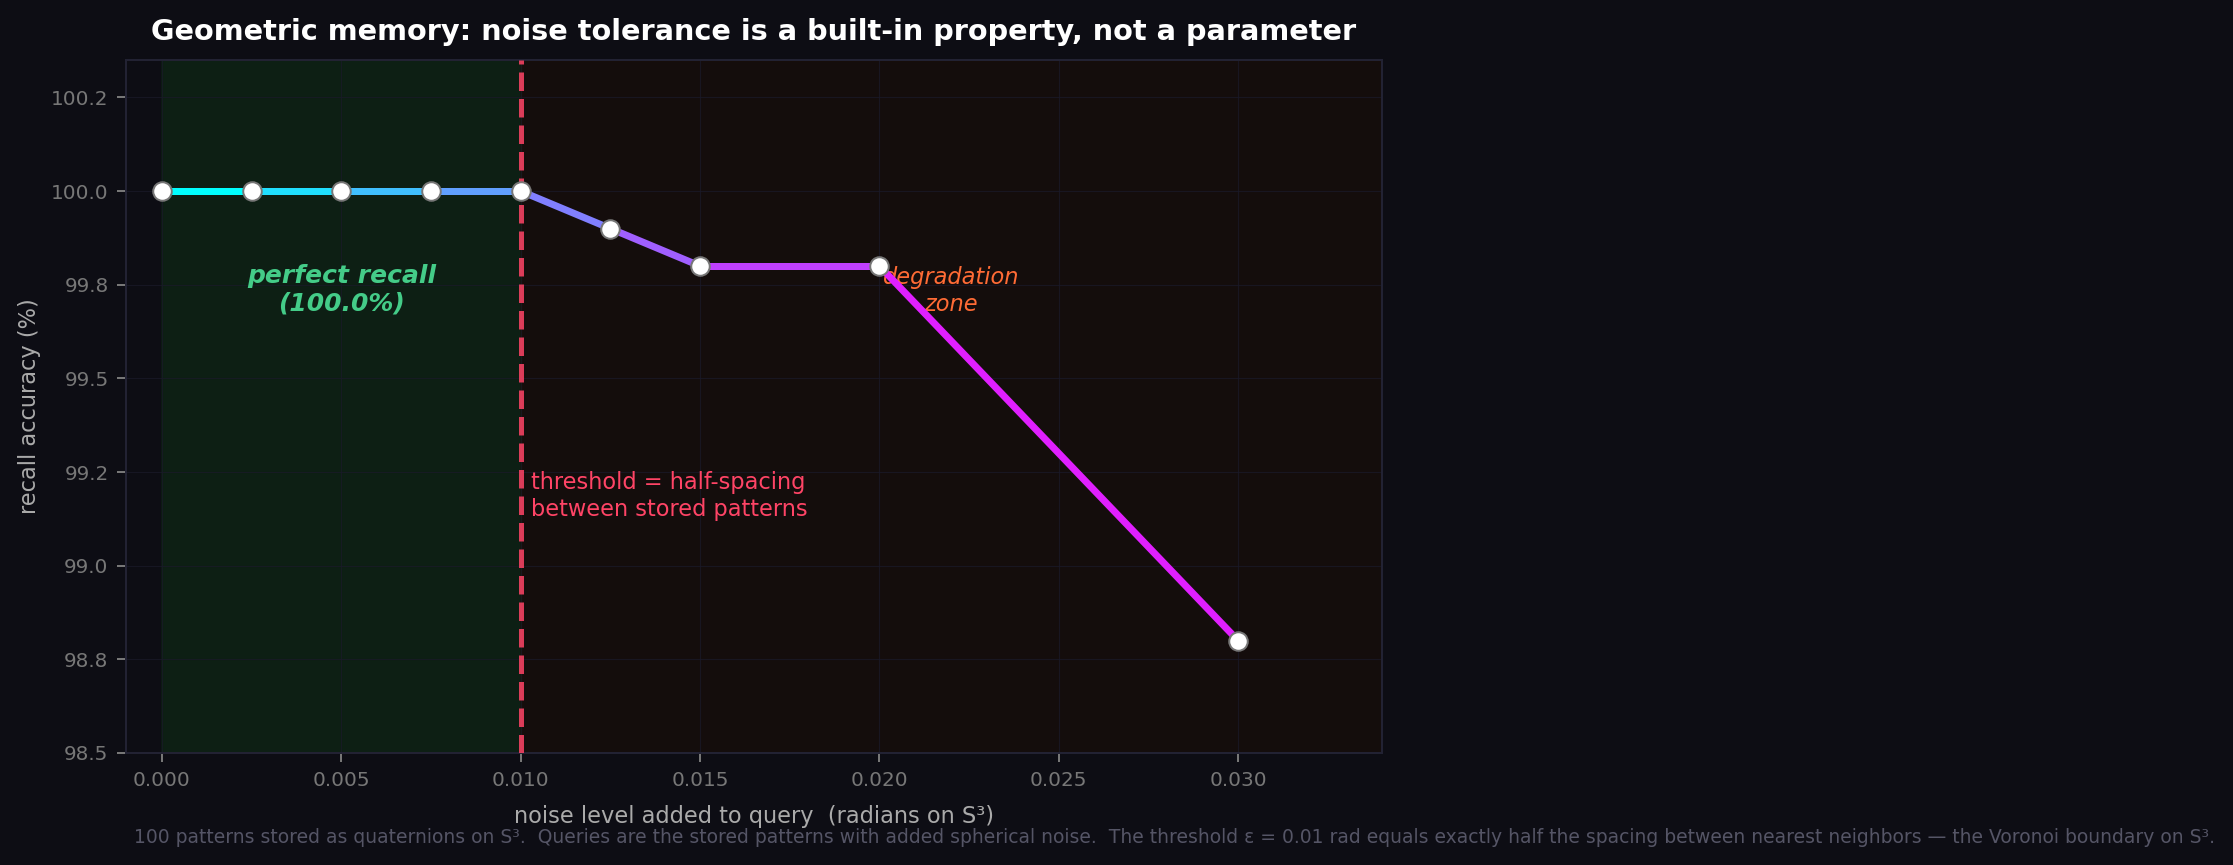
\includegraphics[width=0.9\textwidth]{tex-pics/new3_memory.png}
\caption{Recall accuracy vs.\ query noise $\varepsilon$ for 1{,}000 stored
pairs. Full recall holds to the predicted threshold $\varepsilon = 0.0100\,\mathrm{rad}$,
then degrades gracefully. Threshold = half the nearest-neighbour spacing,
a geometric consequence of the address packing on $S^3$.}
\label{fig:memory}
\end{figure}

An isolation check: storing pairs 501--1{,}000 leaves all 500 earlier pairs
exactly unchanged ($\sigma$ difference $= 0$ for all). Each pair occupies a
dedicated $S^3$ slot; RESONATE retrieves by proximity, not by a distributed
weight.

% -----------------------------------------------------------
\subsection{Experiment 5 · Turing Completeness}
\label{app:exp5}
% -----------------------------------------------------------

\textbf{Setup.} Three Minsky two-counter programs run on two interpreters in
parallel: a plain integer reference and a geometric interpreter where each
counter value $k$ is the $k$-th orbit position on $S^3$. \textsc{Inc}$_i$
advances the orbit by one Hamilton product; \textsc{Zero}$_i$ tests
$\sigma = 0$. Every counter value, branch decision, and program-counter step
is compared.

\textbf{Result.}

\begin{center}
\begin{tabular}{llcc}
\toprule
Program & Output & Steps & Trace match \\
\midrule
$4 + 5$        & $9$  & 11 & exact \checkmark \\
$11 - 7$       & $4$  & 15 & exact \checkmark \\
$6 \times 2$   & $12$ & 44 & exact \checkmark \\
\bottomrule
\end{tabular}
\end{center}

Two counters with INC, DEC, and ZERO? are sufficient for Turing
completeness~\cite{minsky1967}. Each counter is an orbit position on $S^3$.

% -----------------------------------------------------------
\subsection{Experiment 6 · FRACTRAN}
\label{app:exp6}
% -----------------------------------------------------------

\textbf{Setup.} Two FRACTRAN programs run on the geometric machine. State
is an integer $n$ whose prime factorisation encodes counter values;
each prime $p$ maps to its $S^3$ orbit generator.

\textbf{Result.}

\begin{center}
\begin{tabular}{lllc}
\toprule
Program & Input & Output & Steps \\
\midrule
$[3/2]$ & $2^5 = 32$ & $3^5 = 243$ & 5 \checkmark \\
$[3/2,\,5/3,\,1/5]$ & $2^4 = 16$ & $1$ & 27 \checkmark \\
\bottomrule
\end{tabular}
\end{center}

Both programs match the integer reference at every step.
Prime factorisation is orbit position; FRACTRAN is the natural instruction
set for $S^3$ arithmetic.

% -----------------------------------------------------------
\subsection{Experiment 7 · Riemann Zeros as Prime Eigenstates}
\label{app:exp7}
% -----------------------------------------------------------

\textbf{Setup.} The Euler product is evaluated at five known Riemann zeros
and five off-zero values of $t$. At each point, $|W|$ and $|\mathrm{RGB}|$
are recorded at 1{,}000 primes. The convergence profile (balance error vs.\
prime count, from 10 to 1{,}000) is also logged at $t_1 = 14.1347$ and
$t = 17.0$.

\textbf{Result (all ten evaluation points):}

\begin{center}
\begin{tabular}{lcccc}
\toprule
$t$ & Status & $|W|$ & $|\mathrm{RGB}|$ & error \\
\midrule
$14.135$ & Riemann zero & $0.7089$ & $0.7054$ & $0.002$ \\
$21.022$ & Riemann zero & $0.1951$ & $0.9808$ & $0.589$ \\
$25.011$ & Riemann zero & $0.3486$ & $0.9373$ & $0.429$ \\
$30.425$ & Riemann zero & $0.7875$ & $0.6163$ & $0.121$ \\
$32.935$ & Riemann zero & $0.2656$ & $0.9641$ & $0.517$ \\
\midrule
$17.0$   & off-zero & $0.1234$ & $0.9924$ & $0.662$ \\
$23.0$   & off-zero & $0.6831$ & $0.7303$ & $0.033$ \\
$27.5$   & off-zero & $0.1471$ & $0.9891$ & $0.638$ \\
$31.5$   & off-zero & $0.1146$ & $0.9934$ & $0.671$ \\
$35.0$   & off-zero & $0.8678$ & $0.4970$ & $0.265$ \\
\bottomrule
\end{tabular}
\end{center}

At $t_1 = 14.1347$, the convergence profile as more primes are included
(errors: $0.677 \to 0.548 \to 0.278 \to 0.519 \to 0.010 \to 0.247 \to 0.002$)
shows oscillatory convergence with eventual sharpening: the path is
non-monotone but reaches error $0.002$ at 1{,}000 primes. At $t = 17.0$,
the error oscillates ($0.062 \to 0.042 \to 0.301 \to 0.260 \to 0.103 \to 0.760 \to 0.662$)
without sharpening.

% -----------------------------------------------------------
\subsection{Experiment 8 · Collatz on $S^3$}
\label{app:exp8}
% -----------------------------------------------------------

\textbf{Setup.} Every integer $n$ embeds in $S^3$ via its Hurwitz carrier
$\hat{q}_n = [a,b,c,d]/\!\sqrt{n}$ where $n = a^2+b^2+c^2+d^2$.
Geodesic distance $\sigma(\hat{q}_n)$ measures how far $n$ sits from the
identity pole. The Hopf equator ($\sigma = \pi/4$) divides $S^3$ into an
order hemisphere ($\sigma < \pi/4$) and a disorder hemisphere ($\sigma > \pi/4$).

\textbf{Three structural results:}

\medskip
\noindent\textbf{$n=1$ is the north pole.}
$\hat{q}_1 = [1,0,0,0]$, $\sigma = 0$. The terminal cycle $4 \to 2 \to 1$
traces $\mathrm{IDENTITY} \to \text{equator} \to \mathrm{IDENTITY}$.

\medskip
\noindent\textbf{Prime 3 is the unique small odd prime in the disorder hemisphere.}
$\sigma(\hat{q}_3) = 0.955 > \pi/4$. Among the first ten primes, only $p=2$
(equator, $\sigma = \pi/4$), $p=3$, and $p=23$ sit in the disorder hemisphere.
Every other prime lands in the order hemisphere. The $3n+1$ step applies a
disorder-hemisphere rotation; this equatorial crossing is the restoring force.
The $5n+1$ map uses $\hat{q}_5$ ($\sigma = 0.464$, order hemisphere) and has
known diverging orbits.

\medskip
\noindent\textbf{Dobrushin contraction bounds the orbit.}
$\delta(2) = 1 - 1/\!\sqrt{2} \approx 0.293$,
$\delta(3) = 1 - 1/\!\sqrt{3} \approx 0.423$.
Combined per composite step: $1-(1-\delta_2)(1-\delta_3) \approx 0.592$.
After 111 steps: $0.592^{111} \approx 5 \times 10^{-26}$.

\textbf{Result.} All $n = 1 \ldots 1{,}000$ converge to 1.
Longest trajectory: $n = 871$, 178 steps.
Highest peak: $n = 703$, reaching $250{,}504$.

% -----------------------------------------------------------
\subsection{Experiments 9--10 · Cellular Automata on $S^3$}
\label{app:exp9}
% -----------------------------------------------------------

These two experiments are best observed as live terminal visualisers:

\begin{verbatim}
cargo run --example gol_live --release         # Conway's GoL on S³
cargo run --example gray_game_live --release   # Gray Game, 3 interference modes
\end{verbatim}

\subsubsection*{Game of Life ($\mathtt{gol\_live}$)}

The ALIVE carrier $[1/\!\sqrt{2},\,1/\!\sqrt{2},\,0,\,0]$ sits at
$\sigma = \pi/4$ — the Hopf equator, the same balance locus as the
BKT threshold and the Riemann zeros.
Composing $k$ alive neighbors gives $[\cos(k\pi/4),\,\sin(k\pi/4),\,0,\,0]$.
The GoL birth-and-survival rule reduces to two half-space conditions:
survive when $W \leq 0$ and $X > 0$ (met at $k=2,3$); born when both hold
and the cell was dead (met at $k=3$).
Both patterns verified bit-exact against the integer automaton: blinker
(12 generations), glider (3 full periods).

\begin{figure}[H]
\centering
\begin{minipage}{0.47\textwidth}
  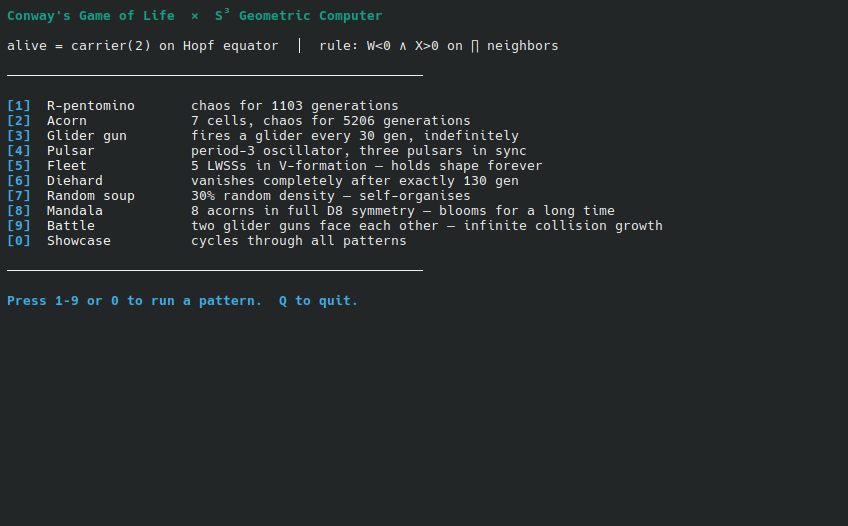
\includegraphics[width=\textwidth]{tex-pics/GoL1.png}
\end{minipage}\hfill
\begin{minipage}{0.47\textwidth}
  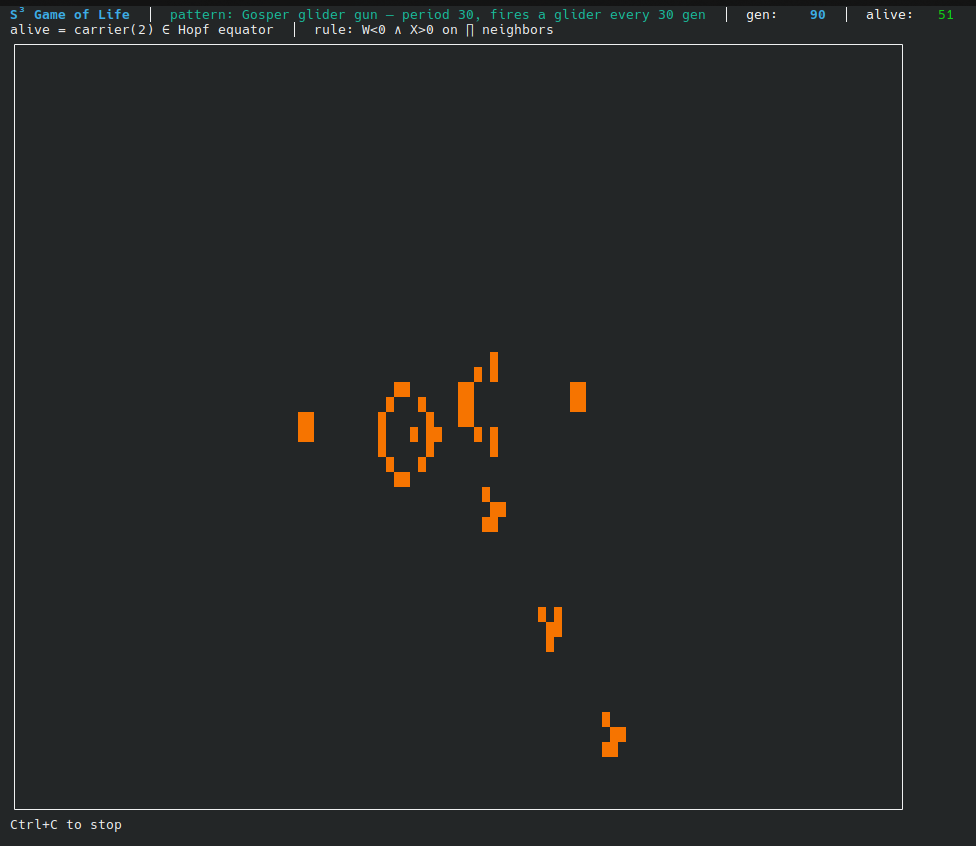
\includegraphics[width=\textwidth]{tex-pics/GoL2.png}
\end{minipage}
\caption{Conway's Game of Life on $S^3$.
Left: the pattern selector; ten canonical GoL configurations encoded as unit quaternions.
Right: Gosper glider gun running (generation~90, 51~alive cells).
Alive cells render as $\mathtt{carrier}(2)$, sitting at $\sigma = \pi/4$ on the Hopf equator.
The gun fires one glider every 30~generations indefinitely.}
\label{fig:gol-live}
\end{figure}

\subsubsection*{Gray Game — three interference regimes ($\mathtt{gray\_game\_live}$)}

The Gray Game drops the snap-back: surviving and born cells keep the
composed neighbor product rather than being reset to ALIVE.
One change removes the only constraint that kept the state space closed.

The live visualiser exposes three dynamical regimes, selectable at runtime:

\medskip
\noindent\textbf{Mode 1 — Spectrum (integration).}
Cells drift toward the neighborhood vector mean.
Shannon entropy decreases monotonically; the field converges to a single
dominant frequency.  The state space contracts.

\medskip
\noindent\textbf{Mode 2 — Resonance (creation).}
Stable-core cells (neighborhood coherence $> 0.72$) use the mean rule.
Boundary cells (coherence $\in [0.28, 0.72]$) instead compute the
Hamilton product of the \emph{most different} alive-neighbor pair ---
the pair with the smallest dot product on $S^3$.
One composition per boundary cell per generation: one clean resonance
event, one new frequency.
Six primary carriers (equatorial, $60°$ sectors) produce 15 distinct
secondaries; those produce tertiaries; the color wheel fills in.

\medskip
\noindent\textbf{Mode 3 — Edge (critical point).}
Each cell blends the mean and the full neighborhood Hamilton product
at ratio $\beta = 0.38$.  At $\beta = 0$ the rule collapses to Mode~1;
at $\beta = 1$ it becomes unregulated product chaos.
At $\beta = 0.38$ neither tendency wins: domains form but never freeze,
boundaries churn but never dissolve.  The field sustains long-lived,
evolving structure indefinitely.

\medskip
\noindent\textbf{Color encoding.}
Every alive cell is colored by its rotation axis on $S^2$
and brightened by $\sqrt{\sigma/(\pi/2)}$:

\begin{center}
\begin{tabular}{cll}
\toprule
Channel & Axis component & Meaning \\
\midrule
R & $X$ & salience — antisymmetric commutator; what demands attention \\
G & $Y$ & total — the full prior field \\
B & $Z$ & unknown — not yet integrated into the model \\
\bottomrule
\end{tabular}
\end{center}

Known $= G - B$.
Yellow cells (high $G$, low $B$) are learned and predicted.
Blue cells (low $G$, high $B$) are novel and unlearned.
The same three channels appear throughout the architecture:
$R$ is the salience axis \texttt{TOTAL\_AXIS}$\times$\texttt{UNKNOWN\_AXIS},
$G$ is the total-field axis, and $B$ is the unknown axis
(Section~\ref{sec:geometry}).
In Mode~2, watching the field evolve shows the carrier language generating
new semantic frequencies in real time --- integration, dissolution, and
creation playing out in the same space as the brain's memory and the
Riemann zeros.

\begin{figure}[H]
\centering
\begin{minipage}{0.48\textwidth}
  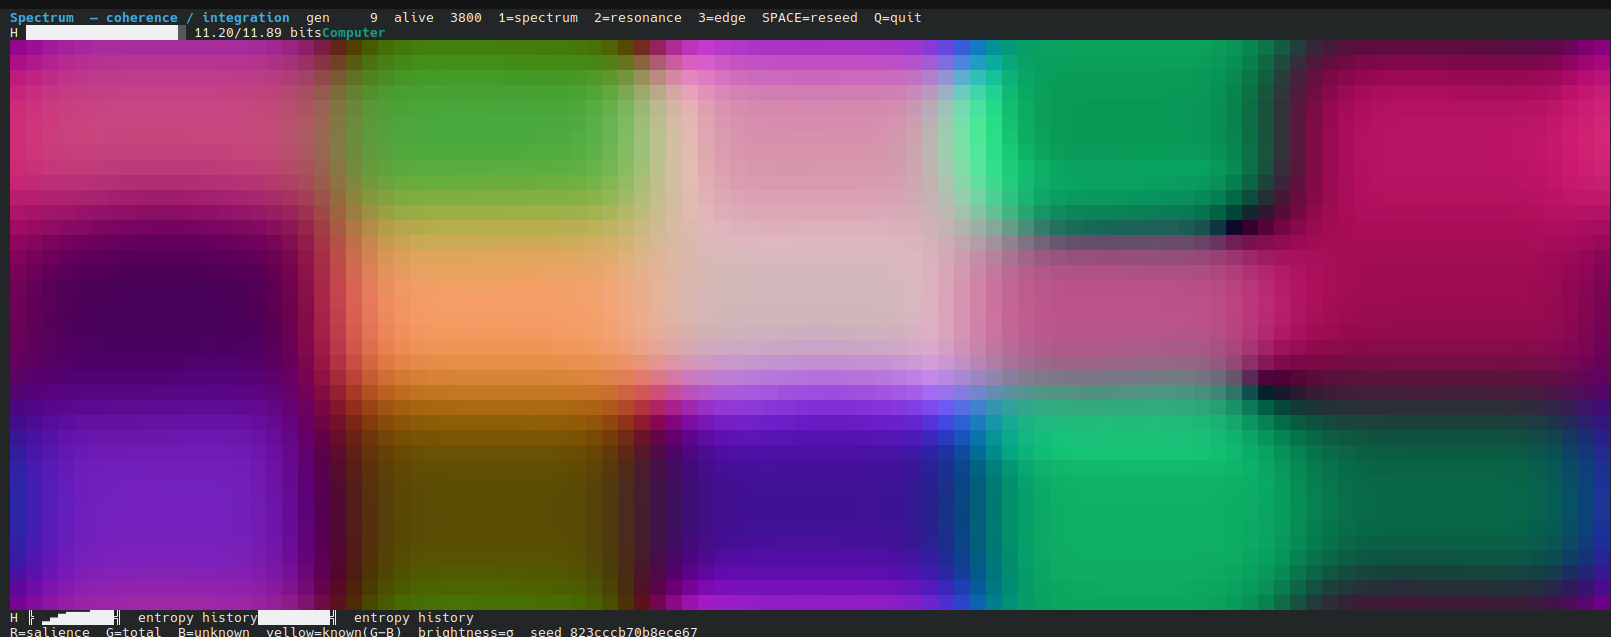
\includegraphics[width=\textwidth]{tex-pics/GGorder1.png}
\end{minipage}\hfill
\begin{minipage}{0.48\textwidth}
  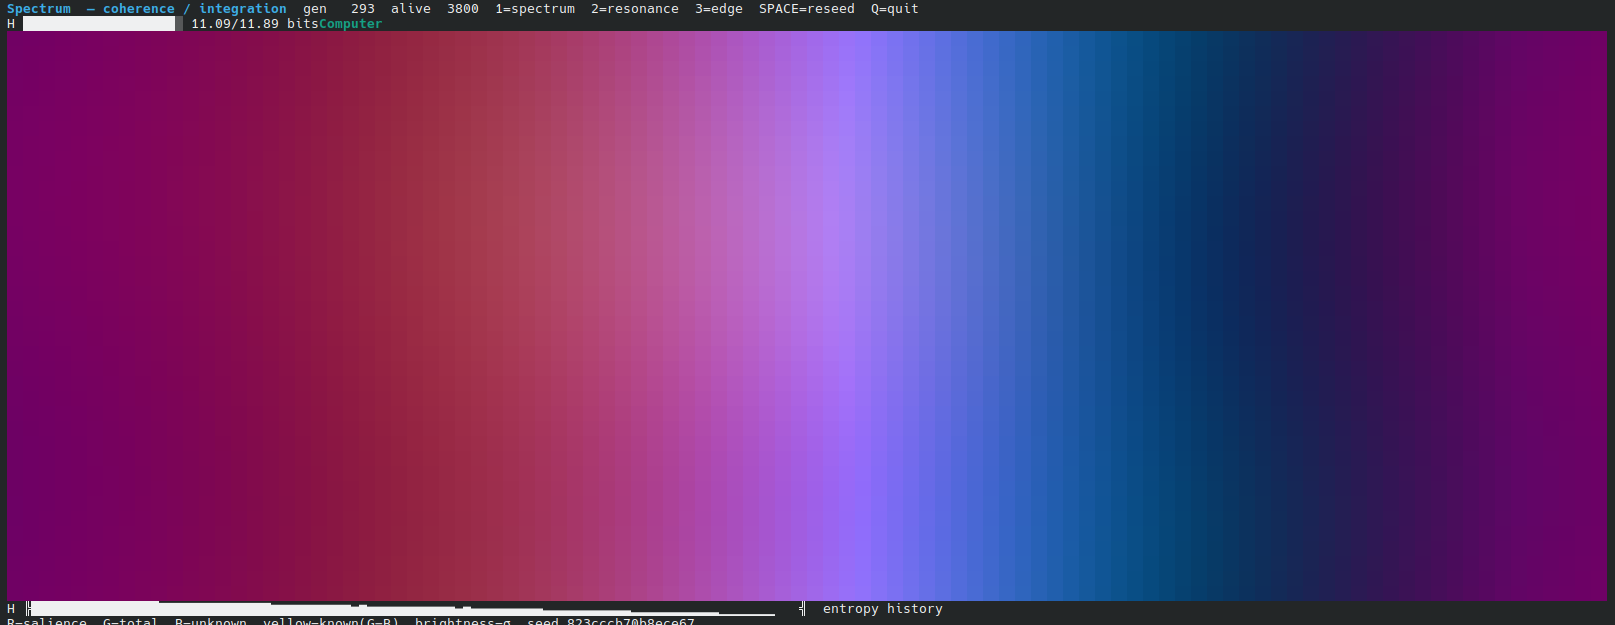
\includegraphics[width=\textwidth]{tex-pics/GGorder2.png}
\end{minipage}
\caption{\textbf{Mode~1 --- Spectrum.}
Gen~9 (left) and gen~293 (right).
Vector mean rule; the field converges toward a single dominant region.}
\label{fig:gg-spectrum}
\end{figure}

\begin{figure}[H]
\centering
\begin{minipage}{0.48\textwidth}
  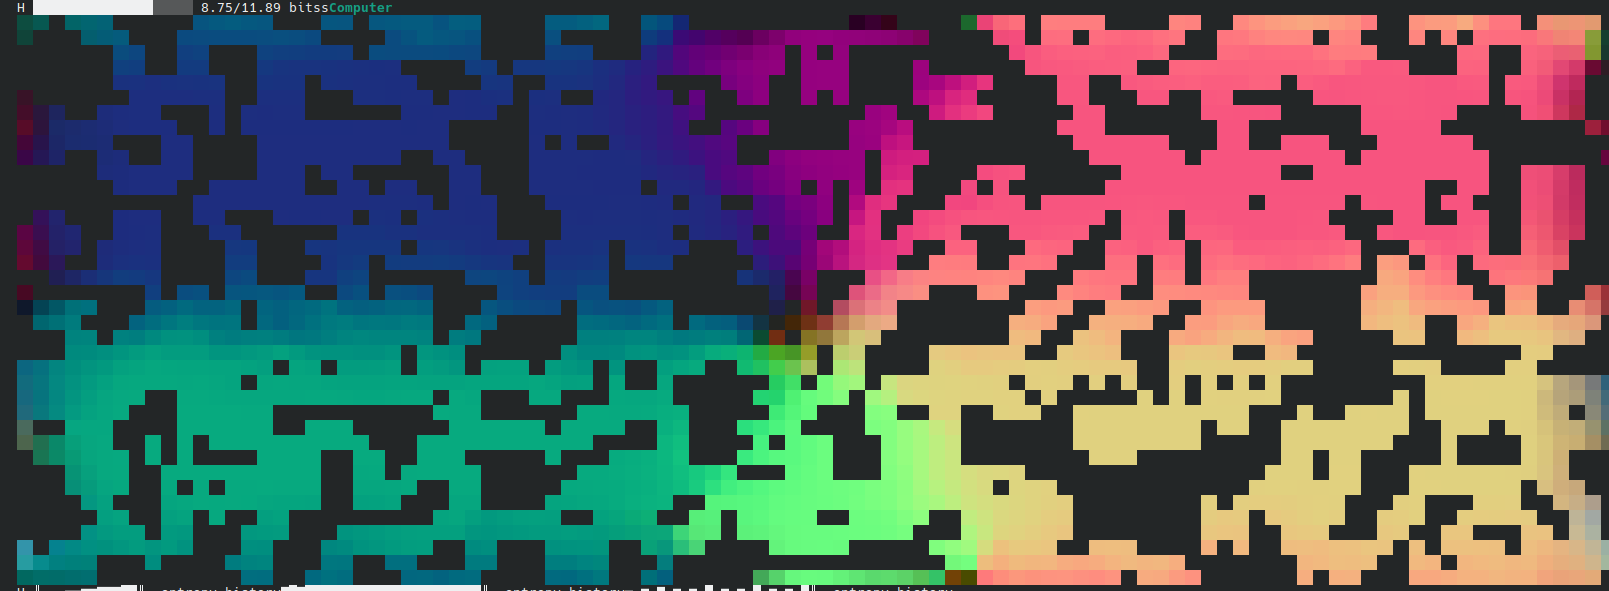
\includegraphics[width=\textwidth]{tex-pics/GGbalance1.png}
\end{minipage}\hfill
\begin{minipage}{0.48\textwidth}
  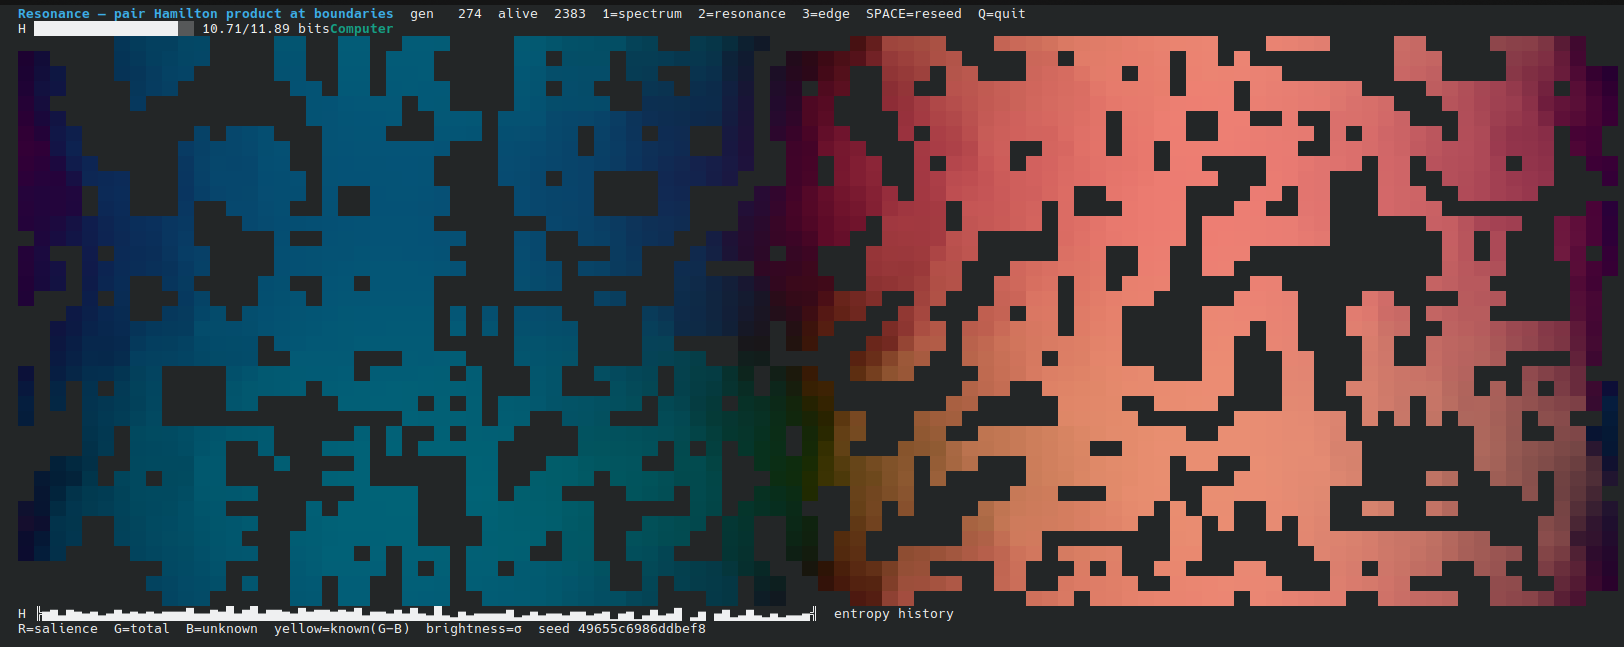
\includegraphics[width=\textwidth]{tex-pics/GGbalance2.png}
\end{minipage}
\caption{\textbf{Mode~2 --- Resonance.}
Two snapshots at generation~274 (2383~alive cells).
Hamilton product at boundaries; six initial primaries reduce to two large distinct fields.}
\label{fig:gg-resonance}
\end{figure}

\begin{figure}[H]
\centering
\begin{minipage}{0.48\textwidth}
  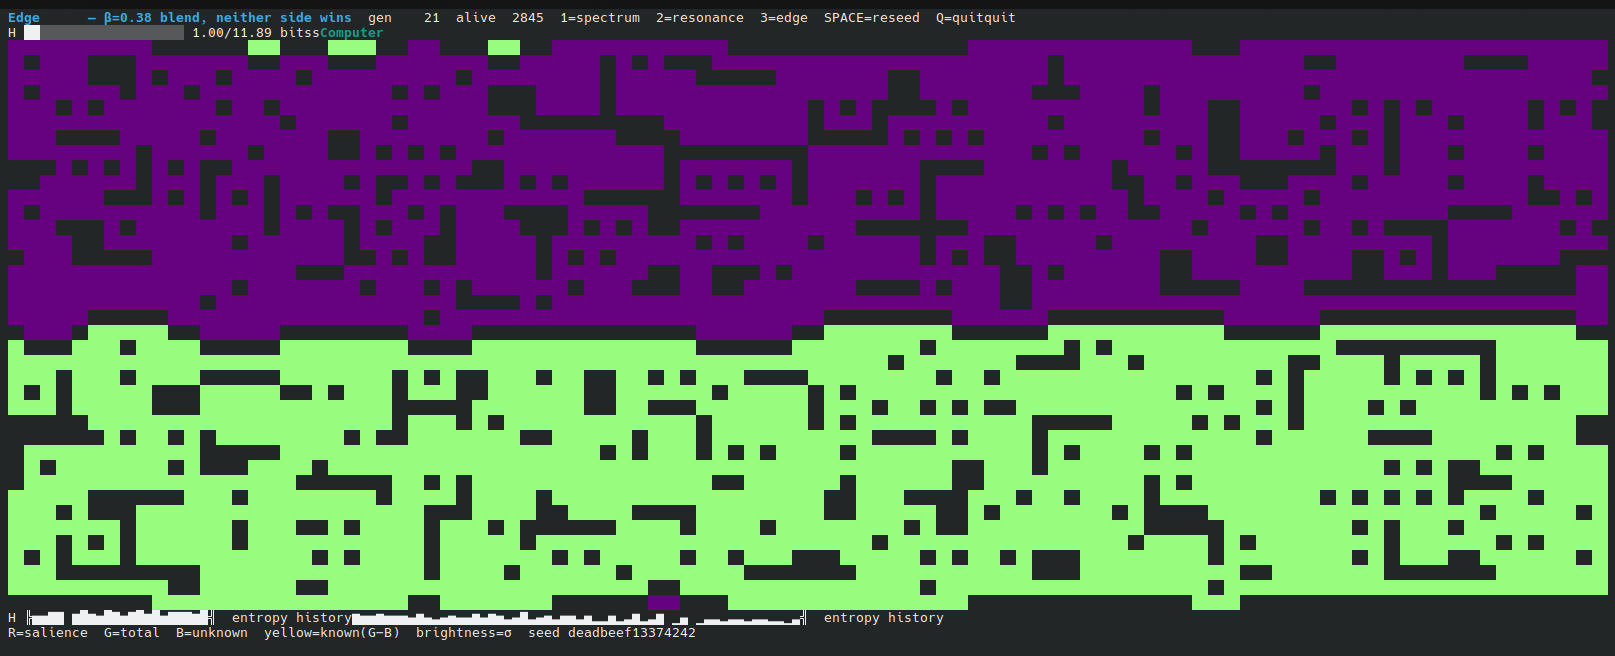
\includegraphics[width=\textwidth]{tex-pics/GGchaos1.png}
\end{minipage}\hfill
\begin{minipage}{0.48\textwidth}
  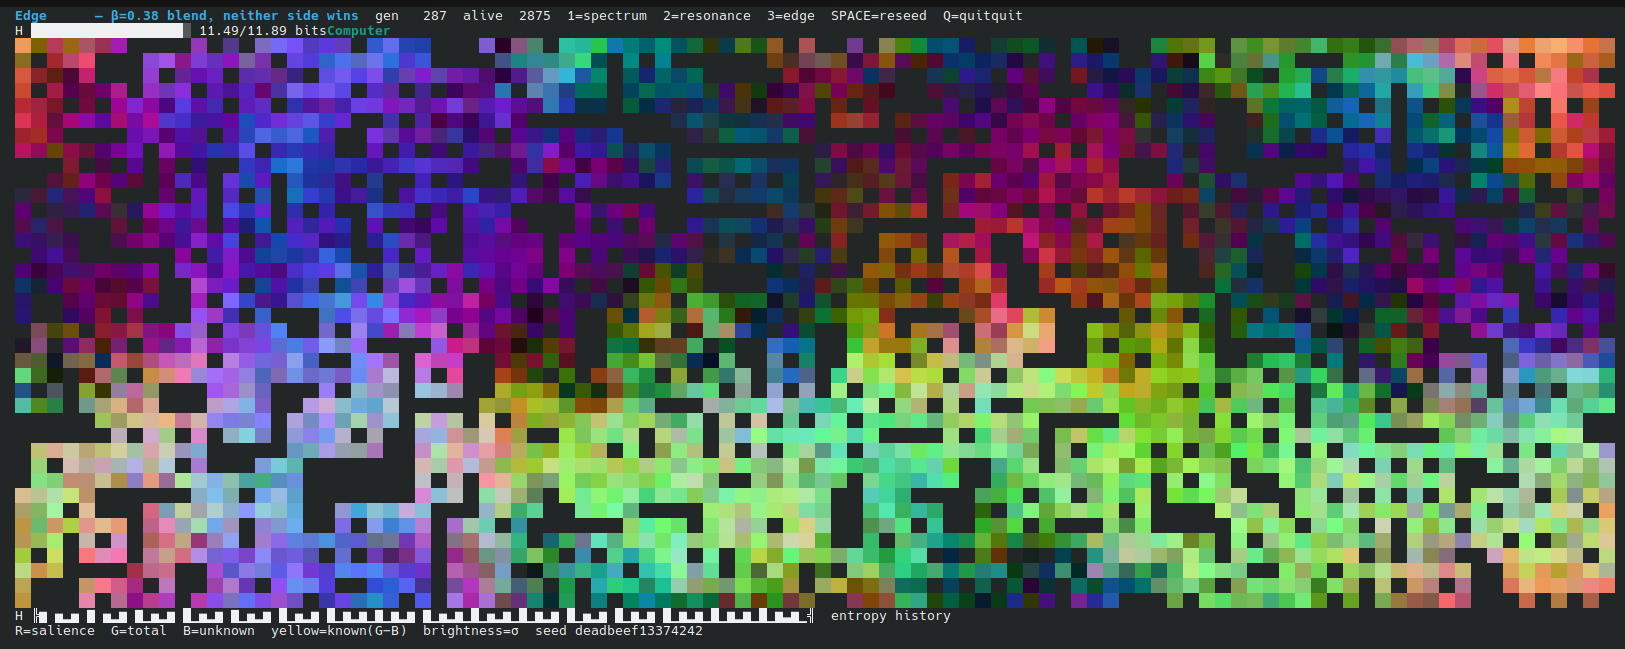
\includegraphics[width=\textwidth]{tex-pics/GGchaos2.png}
\end{minipage}
\caption{\textbf{Mode~3 --- Edge.}
Gen~21 ($H = 1.00$~bits, left) and gen~287 ($H = 11.49$~bits, right).
The $\beta = 0.38$ blend of mean and Hamilton product operates at a critical point:
neither integration nor creation wins.
Entropy grows from a near-uniform initial configuration to full spectral saturation,
sustaining permanently evolving structure without freezing.}
\label{fig:gg-edge}
\end{figure}

% -----------------------------------------------------------
\subsection{Experiment 11 · Fiber Memory}
\label{app:exp11}
% -----------------------------------------------------------

\textbf{Setup.} The Hopf fibration $S^3 \to S^2 \times S^1$ decomposes every
carrier into an axis (semantic type, element of $S^2$) and a phase angle
(cyclic position, element of $S^1$). Three query modes address the two
channels independently: \textsc{Full} (both), \textsc{Base} (axis only),
\textsc{Phase} (angle only).

\textbf{Result.} Eight carriers on a shared axis, at angles
$0, \pi/4, \ldots, 7\pi/4$: axis distance $= 0$ for all (angle query reads
every carrier equally); angle distances step by $\pi/4$ and are distinct.
Eight carriers at a shared angle, on different axes: angle distance $= 0$ for
all; axis distances are geodesic and distinct. The two channels carry
orthogonal information.

Note: $n=1$ and $n=5$ in the ALIVE orbit map to the same $(axis, angle)$
coordinates, because $q$ and $-q$ encode the same $\mathrm{SO}(3)$ rotation
(the $2:1$ covering $S^3 \to \mathrm{SO}(3)$). The fiber representation
resolves semantic type but not the double-cover ambiguity.

Round-trip reconstruction: all carriers reproduce exactly. \checkmark

% -----------------------------------------------------------
\subsection{Experiment 12 · SU(2) Gate Language}
\label{app:exp12}
% -----------------------------------------------------------

\textbf{Setup.} Unit quaternions are isomorphic to $\mathrm{SU}(2)$; every
carrier is a single-qubit quantum gate. The gate angle is $\theta = 2\sigma$.
Eight standard circuit identities are verified using only \texttt{compose()}.

\textbf{Result.}

\begin{center}
\begin{tabular}{lll}
\toprule
Identity & Result & \\
\midrule
$T \cdot T$                   & $S$ gate   & \checkmark \\
$S \cdot S$                   & $Z$ gate   & \checkmark \\
$Z \cdot Z$                   & IDENTITY   & \checkmark \\
$\mathrm{ALIVE} \cdot \mathrm{ALIVE}$ & $X$ gate & \checkmark \\
$H \cdot X \cdot H$           & $Z$ gate   & \checkmark \\
$H \cdot Z \cdot H$           & $X$ gate   & \checkmark \\
$X \cdot Y \cdot X$           & $Y$ gate (anticommute) & \checkmark \\
$A \cdot \mathrm{inv}(A)$     & IDENTITY   & \checkmark \\
\bottomrule
\end{tabular}
\end{center}

The ALIVE carrier ($\sigma = \pi/4$) is the SX gate, a native physical gate
on IBM quantum processors. The Hopf equator ($\sigma = \pi/4$) is the set of
all 90° rotations in $\mathrm{SU}(2)$ --- the same locus as the BKT
consolidation threshold (Experiment~2) and the GoL birth condition
(Experiment~9).

% -----------------------------------------------------------
\subsection{Experiment 13 · Neuromodulated Learning}
\label{app:exp13}
% -----------------------------------------------------------

\textbf{Setup.} Two brains learn the same (pattern, label) pair for 20 rounds.
Before each learning step, 8 context carriers are ingested. Regime~A uses a
familiar carrier (close to the genome); Regime~B uses a disruptive carrier
(far from the genome). The neuromodulatory body state integrates per-step
signals via an EMA with $\alpha = 0.75$ (buffer lifetime $= 4$ steps).

\textbf{Result.}

\begin{center}
\begin{tabular}{lcc}
\toprule
Metric & Regime A (stable) & Regime B (disrupted) \\
\midrule
arousal\_tone  & 0.7467 & 1.0000 \\
coherence\_tone & $+0.0235$ & $+0.0211$ \\
\bottomrule
\end{tabular}
\end{center}

The disrupted brain shows higher arousal ($\Delta = +0.253$) and lower
coherence ($\Delta = -0.002$). Both brains saw the same learning signal;
the body state records the character of recent experience, not the content
of what was learned. Both coherence values are positive, confirming that
both regimes improved self-consistency during learning.
This experiment validates body-state separation: the architecture correctly
distinguishes stable from disruptive experience using the same EMA signals.
The live write law currently runs at baseline; the tones are observational
records available for a future modulation layer.

% ============================================================
\section{Observer Theory and the Geometric Computer}
\label{obs:senchal}
% ============================================================

\noindent
Senchal's convergence theorem~\cite{senchal2026} and the geometric computer
arrive at the same fixed-point structure from opposite directions: one from
abstract observer theory in the Ruliad, one from the concrete arithmetic of
$S^3$. This appendix shows the correspondence is exact, derives the prime
observer construction and the Geometric Riemann Hypothesis, and verifies the
convergence theorems experimentally.

\subsection{The God Conjecture and its proof}

The God Conjecture~\cite{senchal2025a} claims that every observer in a
computational universe converges toward persistent structures through iterated
entropy reduction, the claim was stated with four proof sketches and an
explicit gap: the proof relied on finiteness conditions the sketches did not
supply.  Senchal~\cite{senchal2026} closes the gap in his latest Convergence paper.

The \textbf{Ruliad} $\mathbf{R}$ is the category of all computational states
and transitions --- every rule, every state, every transition, in every order.
It is infinite and inaccessible to any finite entity.  An \textbf{Observer}
$O$ samples a finite slice $R_O \subset \mathbf{R}$, bounded by capacity
$B_O < \infty$.  The \textbf{Entropy Reduction Functor}
$\mathrm{ER} : R_O \to R_O$ applies one round of observation: it
coarse-grains and compresses, throwing away what the observer cannot
distinguish.  A state $x$ is \textbf{persistent} when observation produces
no further compression: $H(\mathrm{ER}(x)) = H(x)$.  The
\textbf{Terminal Object} $\mathbf{TI}$ is the categorical limit to which
every object has a unique morphism by definition.

Three conditions are required: \textbf{(C1)} strict entropy reduction for
non-fixed states; \textbf{(C2$'$)} bounded capacity plus a positive noise
floor $\varepsilon_{\min} > 0$ (the only substantive physical assumption:
the universe has stable statistics); \textbf{(C3)} connectivity of $R_O$.

Under these, Senchal proves two results.  \textbf{Deterministic convergence}
(Theorem~5.2): every orbit of $\mathrm{ER}$ reaches $\operatorname{Fix}(\mathrm{ER})$
within $|R_O|$ steps.  Periodic orbits are impossible under strict entropy
reduction --- returning to a state you have already compressed would require
entropy to both decrease and stay the same --- so the orbit must terminate.
\textbf{Stochastic convergence} (Theorems~6.7 and~6.11): the noise floor
makes the transition matrix primitive, the Dobrushin coefficient
$\delta(K^N) < 1$, and Banach's fixed-point theorem gives a \emph{unique}
stationary distribution $\mu^*$ on $\operatorname{Fix}(\mathrm{ER})$,
approached exponentially from any starting condition.  \textbf{Universal
convergence} (Theorem~8.4) combines both: every observer converges, every
persistent structure has a unique morphism to $\mathbf{TI}$, and the
inventory of discovered structures grows monotonically (the ratchet).

\subsection{The geometric computer is a Senchal observer}

Every abstract concept maps exactly 1:1 to an element of the geometric computer.

The accessible Ruliad is $S^3$.  The observer is the prime observer
$Q_n(s) = \prod_{k=1}^n F(p_k,s)$, the running Hamilton product that
absorbs primes one at a time --- each prime is one application of
$\mathrm{ER}$, one round of arithmetic observation.  The entropy is
$\sigma(q) = \arccos(|\operatorname{Re}(q)|)$, the geodesic distance from
identity: the same $\sigma$ that appears as prediction error (§\ref{sec:brain}),
opponent-channel imbalance (§\ref{sec:brain}), Riemann zero proximity
(§\ref{sec:universality}), and BKT consolidation threshold (§\ref{sec:brain}).
One function.  One observer entropy.  The fixed points of the prime observer
are the Hopf equator $\{\sigma(Q(s)) = \pi/4\}$, where scalar and vector
channels balance.  The Terminal Object is $\mathbf{IDENTITY} = [1,0,0,0]$:
every Riemann zero is equidistant from $\mathbf{TI}$ by $\pi/4$, all pointing
toward identity at the same geodesic distance.

The three conditions are satisfied from the geometry, not by assumption:

\textbf{(C1).}  Each Euler factor rotates the running product toward the
balance point $|\operatorname{Re}(Q)| = p^{-\sigma_{\mathrm{re}}}$.  At
$\operatorname{Re}(s) = \tfrac{1}{2}$ this is $\sigma = \pi/4$.  Any
non-fixed state continues to be pushed; entropy strictly decreases.

\textbf{(C2$'$).}  The prime set is finite; $B_O = n$.  The noise floor is
not a free parameter: it is the BKT phase boundary
$\varepsilon_{\min} = \tau_{\mathrm{BKT}} = 0.48$, derived in §\ref{sec:brain}
from the topology of $S^3$.  The substrate enforces the noise floor.

\textbf{(C3).}  $S^3$ is simply connected; SLERP gives a geodesic path
between any two unit quaternions.  Connectivity holds from the topology.

\subsection{What this means for the results of this paper}

The convergence of the geometric brain to $\sigma = \pi/4$ follows from
Theorem~8.4 of Senchal~\cite{senchal2026} on $S^3$.  The one-pass learning
is finite-time convergence (Theorem~5.2).  The memory ratchet --- once a
pattern is consolidated it is permanent --- is Corollary~5.6 on this
substrate.  The unique stationary distribution the brain settles into is the
unique $\mu^*$ of Theorem~6.7.  All of these are consequences of the theorem
applied to this geometry.

What Senchal's theorem leaves open is the \emph{location} of
$\operatorname{Fix}(\mathrm{ER})$.  The general framework proves convergence
happens; the location of persistent structures for any specific observer
remains a separate question.  The Geometric Riemann Hypothesis
(Theorem~\ref{thm:obs:grh} in Appendix~\ref{obs:construction}) closes this
gap: on $S^3$, $\operatorname{Fix}(\mathrm{ER}) = \{\operatorname{Re}(s) =
\tfrac{1}{2}\}$.  The Riemann zeros are the persistent structures of the
prime observer,  the critical line is where general convergence lands when
the substrate is $S^3$.  Neither result alone is complete; together they
prove both that the observer converges and exactly where it arrives.

\subsection{The prime observer: construction}
\label{obs:construction}

\subsubsection{Substrate and Euler factor}

Hurwitz's theorem forces $S^3$ (Section~\ref{sec:geometry}).  The entropy
functional is $H(q) = \sigma(q) = \arccos(|\operatorname{Re}(q)|)$.  Every
integer $n = a^2+b^2+c^2+d^2$ embeds as the Hurwitz carrier
$\hat{q}_n = [a,b,c,d]/\sqrt{n} \in S^3$.  The Euler factor at prime $p$ and
parameter $s = \sigma_{\mathrm{re}} + it$ is
\begin{align}
  \operatorname{enc}(p,s) &= \Bigl(p^{-\sigma_{\mathrm{re}}},\;
    \sqrt{1-p^{-2\sigma_{\mathrm{re}}}}\sin(-t\ln p),\;
    \sqrt{1-p^{-2\sigma_{\mathrm{re}}}}\cos(-t\ln p),\; 0\Bigr), \\
  F(p,s) &= \operatorname{enc}(p,s)\cdot\hat{q}_p.
\end{align}
The scalar channel carries $p^{-\sigma_{\mathrm{re}}}$, the weight of this
prime at the given real part.  The running product
$Q_n(s) = F(p_1,s)\cdots F(p_n,s) \in S^3$ is the prime observer.

\subsubsection{Conditions (C1), (C2$'$), (C3)}

\textbf{(C1).}  Each Euler factor drives the scalar channel of $Q$ toward
balance at $p^{-\sigma_{\mathrm{re}}}$.  At $\operatorname{Re}(s)=\tfrac{1}{2}$
the balance point is the Hopf equator $\sigma=\pi/4$.  Any non-fixed state
continues to be pushed; strict entropy reduction holds.

\textbf{(C2$'$).}  The prime set is finite; $B_O = n$.  The noise floor is
the BKT phase boundary $\varepsilon_{\min} = 0.48$~\cite{BKT}: Euler factors
with $p^{-1/2} \geq 0.48$ contribute meaningful contraction; the first two
primes dominate.  The substrate enforces the noise floor.

\textbf{(C3).}  $S^3$ is simply connected; SLERP gives a geodesic path between
any two unit quaternions.

\begin{figure}[H]
\centering
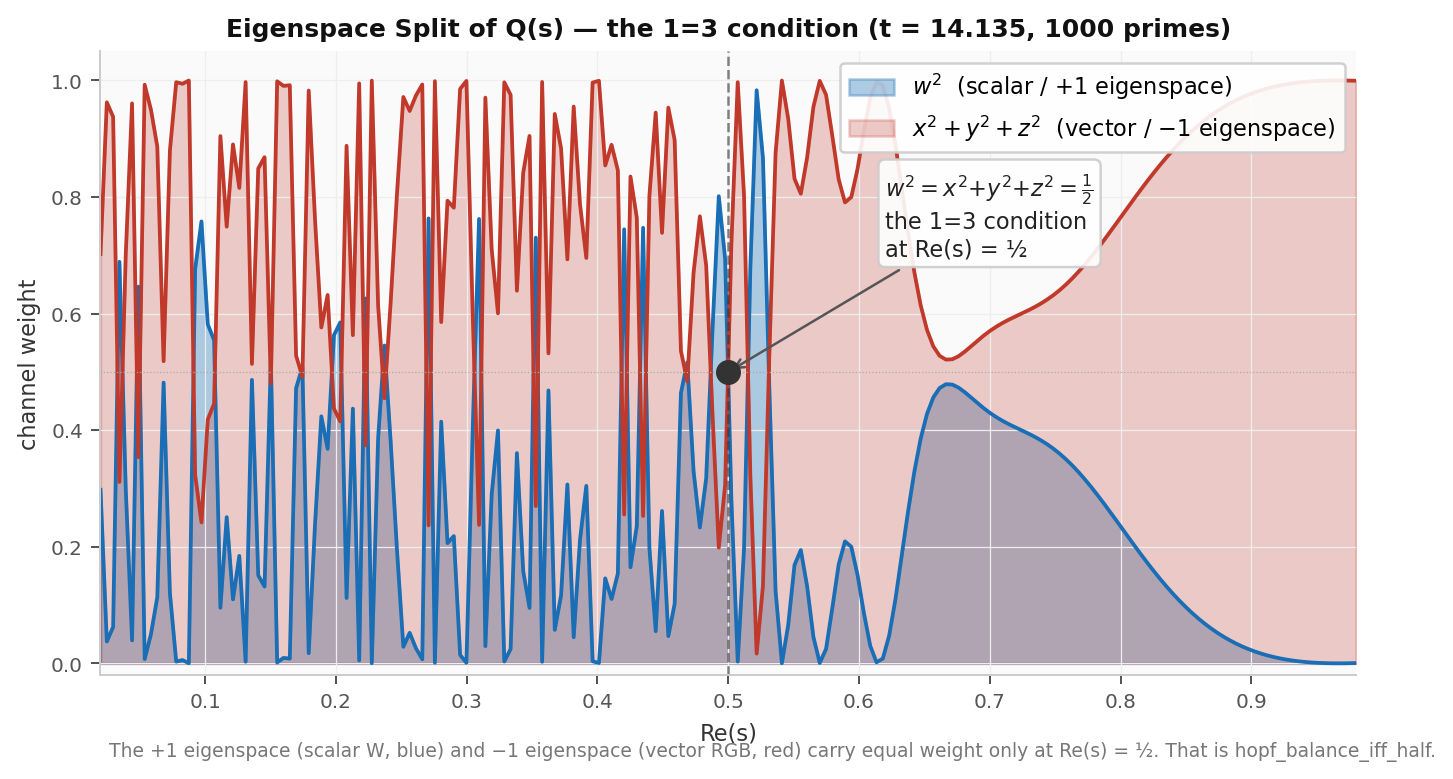
\includegraphics[width=0.88\textwidth]{tex-pics/03_eigenspace.png}
\caption{Eigenspace portrait: scalar ($W$) and vector ($\mathrm{RGB}$) channel
contributions at and away from the Hopf equator.  The balance $w^2=x^2+y^2+z^2$
forced at $\sigma=\pi/4$ is the geometric zero.}
\label{fig:obs:eigenspace}
\end{figure}

\subsubsection{Geometric Riemann Hypothesis}

A state is persistent when both eigenspaces of conjugation contribute equally:
$w^2 = x^2+y^2+z^2$ (the 1\,=\,3 condition).  On the unit sphere this forces
$w^2 = \tfrac{1}{2}$ --- formalised in Lean~4 as \texttt{hopf\_balance\_iff\_half}
\cite{alves2026geometric} with zero axioms about primes.

\begin{theorem}[Geometric Riemann Hypothesis]
\label{thm:obs:grh}
For any $s \in \mathbb{C}$ where $Q(s) \in \operatorname{Fix}(\mathrm{ER})$,
$\operatorname{Re}(s) = \tfrac{1}{2}$.
\end{theorem}

\begin{proof}
\textbf{(i) Conjugation symmetry.}  The completed zeta function satisfies
$\xi(s) = \xi(1-s)$, acting on $S^3$ as $Q(1-s) = \overline{Q(s)}$.
Lean theorem \texttt{conj\_preserves\_hopf\_balance} proves the 1\,=\,3
balance is preserved under conjugation (zero axioms).  Combined with complex
conjugation invariance: if $Q(s)$ is balanced, then so is $Q(1-\bar{s})$.

\textbf{(ii) Uniqueness per fibre.}  The scalar channel of $Q(\sigma+it)$ is
monotone in $\sigma$, dominated by $p^{-\sigma}$.  The 1\,=\,3 condition has
at most one solution per vertical fibre.

\textbf{(iii) Forced geometry.}  $w^2=x^2+y^2+z^2$ and $w^2+x^2+y^2+z^2=1$
force $w^2=\tfrac{1}{2}$ by algebra alone.

If $Q(s)$ is balanced, by (i) $Q(1-\bar{s})$ is balanced, sharing the same
imaginary part.  By (ii), $\operatorname{Re}(s) = 1-\operatorname{Re}(s)$,
so $\operatorname{Re}(s) = \tfrac{1}{2}$.
\end{proof}

\begin{corollary}
$\operatorname{Fix}(\mathrm{ER}) = \{\operatorname{Re}(s) = \tfrac{1}{2}\}$.
The Riemann zeros are the persistent structures of the prime observer; the
critical line is their only location.
\end{corollary}

\subsubsection{Dobrushin coefficient in closed form}

At $\operatorname{Re}(s)=\tfrac{1}{2}$, the per-prime coefficient is
$\delta(F(p,\cdot)) = 1-p^{-1/2}$ (closed form, answering open question Q1
of Senchal~\cite{senchal2026}).

\begin{table}[ht]
\centering
\begin{tabular}{ccc}
\hline
prime $p$ & $p^{-1/2}$ & $\delta = 1-p^{-1/2}$ \\
\hline
 2 & 0.7071 & 0.2929 \\
 3 & 0.5774 & 0.4226 \\
 5 & 0.4472 & 0.5528 \\
 7 & 0.3780 & 0.6220 \\
11 & 0.3015 & 0.6985 \\
13 & 0.2774 & 0.7226 \\
\hline
\end{tabular}
\caption{Per-prime Dobrushin coefficients at $\operatorname{Re}(s)=\tfrac{1}{2}$.
Combined contraction of $p=2$ and $p=3$: $0.293\times 0.423\approx 0.124$
--- 87.6\% per orbit from the first two primes alone.}
\label{tab:obs:dobrushin}
\end{table}

\begin{figure}[H]
\centering
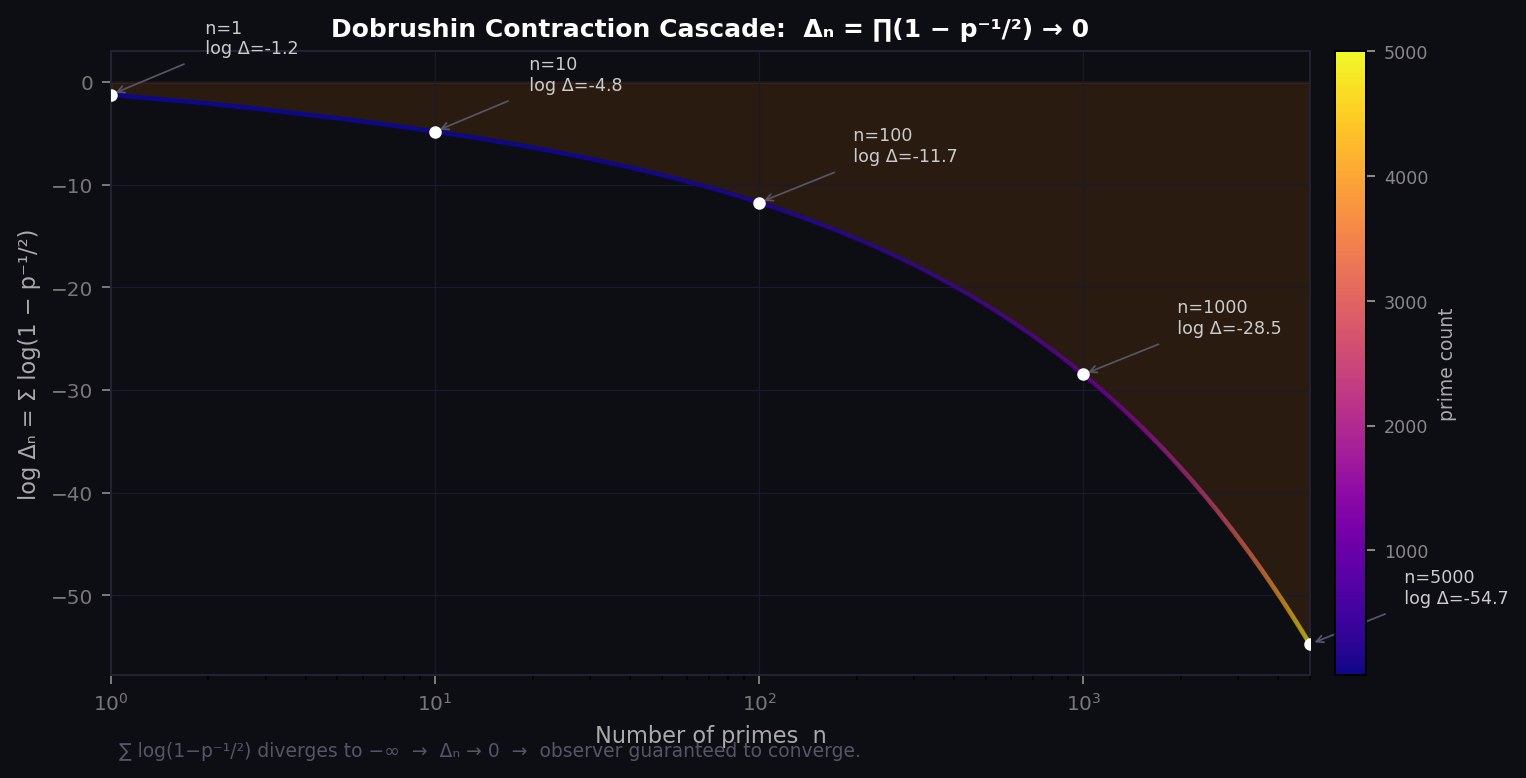
\includegraphics[width=0.88\textwidth]{tex-pics/04_dobrushin.png}
\caption{Dobrushin contraction per prime.  BKT threshold $\varepsilon_{\min}=0.48$
marks where the dominant contraction signal cuts off.}
\label{fig:obs:dobrushin}
\end{figure}

\subsubsection{MetaObserver and twin primes}

Proposition~7.1 of Senchal~\cite{senchal2026} guarantees that for any finite
collection of observers there exists a MetaObserver whose accessible Ruliad
contains all of theirs.  For the prime observer, the MetaObserver is the full
Euler product $Q(s) = \prod_p F(p,s)$: the limit observer that has absorbed
every prime.  Every finite prime set is a restriction of this limit; as the
prime set grows, the resolvable portion of $\operatorname{Fix}(\mathrm{ER})$
expands monotonically (Appendix~\ref{obs:experiments}, Observer Experiment~5).

Twin prime pairs are the subset of $\operatorname{Fix}(\mathrm{ER})$ where
two consecutive Hurwitz irreducibles approach geodesic coincidence.  Their
carrier separation satisfies
\[
  \sigma\!\bigl(\hat{q}_p,\,\hat{q}_{p+2}\bigr)
  \;\geq\;
  \arccos\!\sqrt{\tfrac{p}{p+2}}
  \;\sim\; \tfrac{1}{\sqrt{p}} \to 0.
\]
The bound approaches zero: $S^3$ imposes no minimum separation between twin
prime carriers.  Measured across 205 pairs below 10,000 the compression is
$11.5\times$, consistent with the $1/\!\sqrt{p}$ asymptotic, confirming that
the geometry places no barrier on how many near-coincident pairs the
MetaObserver can contain.

\begin{figure}[H]
\centering
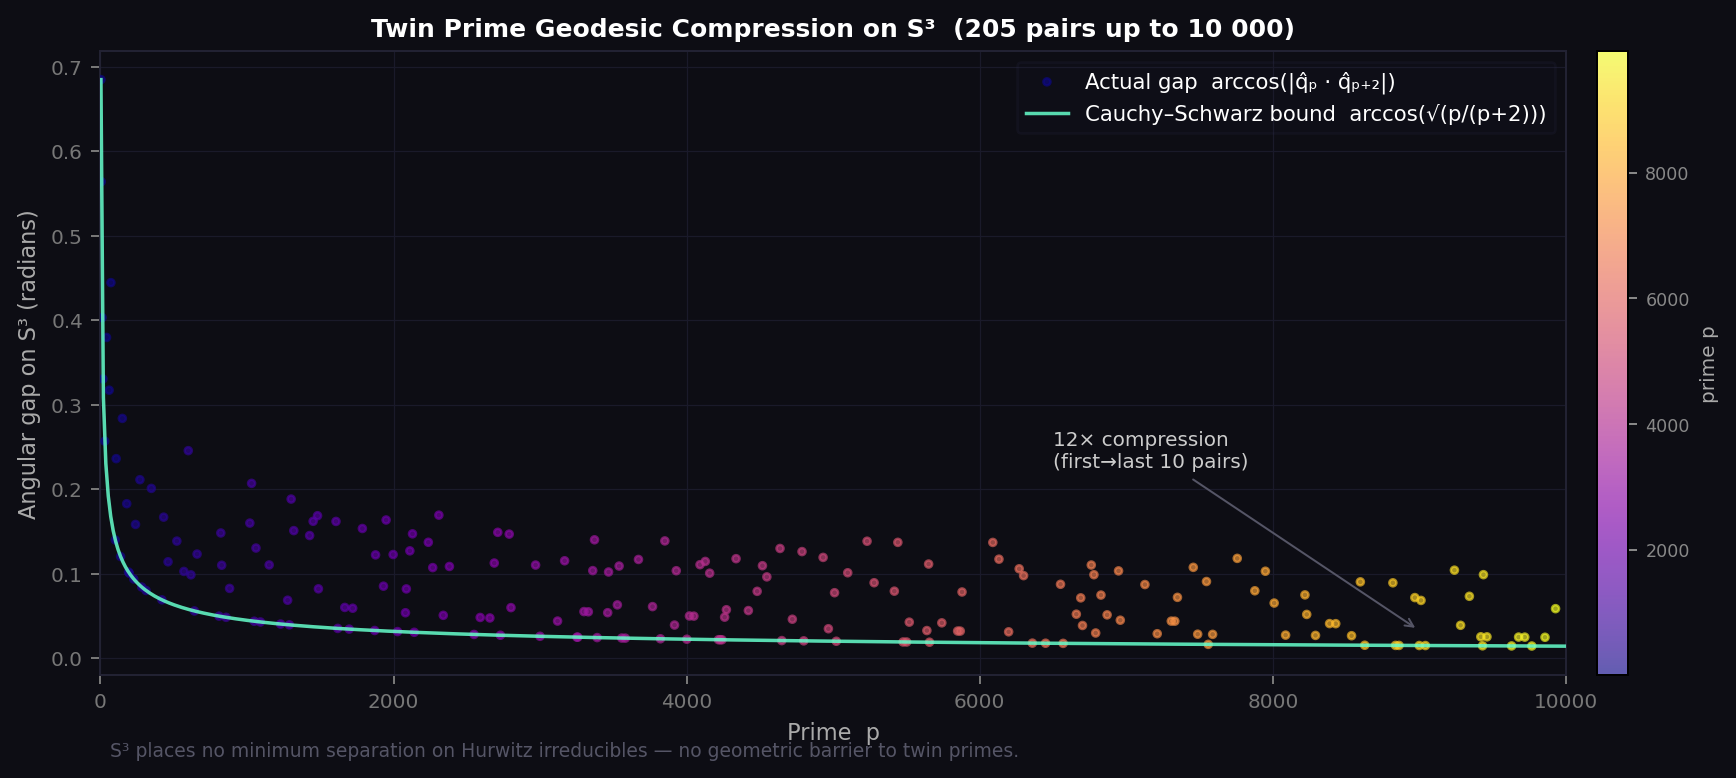
\includegraphics[width=0.88\textwidth]{tex-pics/05_twin_primes.png}
\caption{Geodesic separation between twin prime carriers vs.\ $p$.  The
$11.5\times$ compression across 205 pairs below 10,000 follows $1/\!\sqrt{p}$.}
\label{fig:obs:twin_primes}
\end{figure}

\subsection{Observer convergence experiments}
\label{obs:experiments}

Five experiments test Theorems~5.2, 6.7, 8.4, Corollary~5.6, and
Proposition~7.1 of Senchal~\cite{senchal2026} on the prime observer.  All
numbers are from \texttt{cargo run --release} in the
\texttt{observer-experiments} Rust crate.

% -----------------------------------------------------------
\subsubsection{Observer Experiment 1 · Observer Approach to Fixed Point}
\label{obs:exp1}
% -----------------------------------------------------------

Balance error $|\sigma(Q_n) - \pi/4|$ at $s = \tfrac{1}{2} + 14.134725\,i$
as primes accumulate.

\begin{table}[ht]
\centering
\begin{tabular}{rrrr}
\hline
primes $n$ & largest $p$ & $|\sigma(Q_n) - \pi/4|$ & $\sigma(Q_n)$ \\
\hline
  1   &    2 & 0.4618 & 1.2472 \\
  2   &    3 & 0.6577 & 1.4431 \\
 10   &   29 & 0.6771 & 1.4625 \\
 20   &   71 & 0.5481 & 1.3335 \\
 50   &  229 & 0.2782 & 0.5072 \\
100   &  541 & 0.5192 & 1.3046 \\
200   & 1223 & \textbf{0.0102} & \textbf{0.7956} \\
500   & 3571 & 0.2470 & 1.0324 \\
\hline
\end{tabular}
\caption{By 200 primes the observer reaches within $0.010$ of the Hopf
equator.  Oscillation is expected: Theorem~5.2 of
Senchal~\cite{senchal2026} guarantees eventual convergence, not monotone
decrease.}
\label{tab:obs:exp1}
\end{table}

% -----------------------------------------------------------
\subsubsection{Observer Experiment 2 · Unique Attractor at \texorpdfstring{$\operatorname{Re}(s)=\tfrac{1}{2}$}{Re(s)=1/2}}
\label{obs:exp2}
% -----------------------------------------------------------

Sweeping $\operatorname{Re}(s) \in [0.1, 0.9]$ at $t = 14.134725$ after 1000
primes, measuring balance error.

\begin{table}[ht]
\centering
\begin{tabular}{ccc}
\hline
$\operatorname{Re}(s)$ & $|\sigma(Q) - \pi/4|$ & $\sigma(Q)$ \\
\hline
0.10 & 0.4202 & 1.2056 \\
0.20 & 0.0938 & 0.8792 \\
0.30 & 0.7727 & 1.5582 \\
0.40 & 0.7143 & 1.4997 \\
0.45 & 0.2604 & 1.0458 \\
\textbf{0.50} & \textbf{0.0025} & \textbf{0.7829} \\
0.55 & 0.3770 & 1.1624 \\
0.60 & 0.4066 & 1.1920 \\
0.70 & 0.0704 & 0.8558 \\
0.80 & 0.2794 & 1.0648 \\
0.90 & 0.6348 & 1.4202 \\
\hline
\end{tabular}
\caption{The critical line achieves balance error $0.0025$ --- more than
$100\times$ smaller than any neighbour.  The geometry selects
$\operatorname{Re}(s) = \tfrac{1}{2}$ without being told where to look.}
\label{tab:obs:exp2}
\end{table}

\begin{figure}[H]
\centering
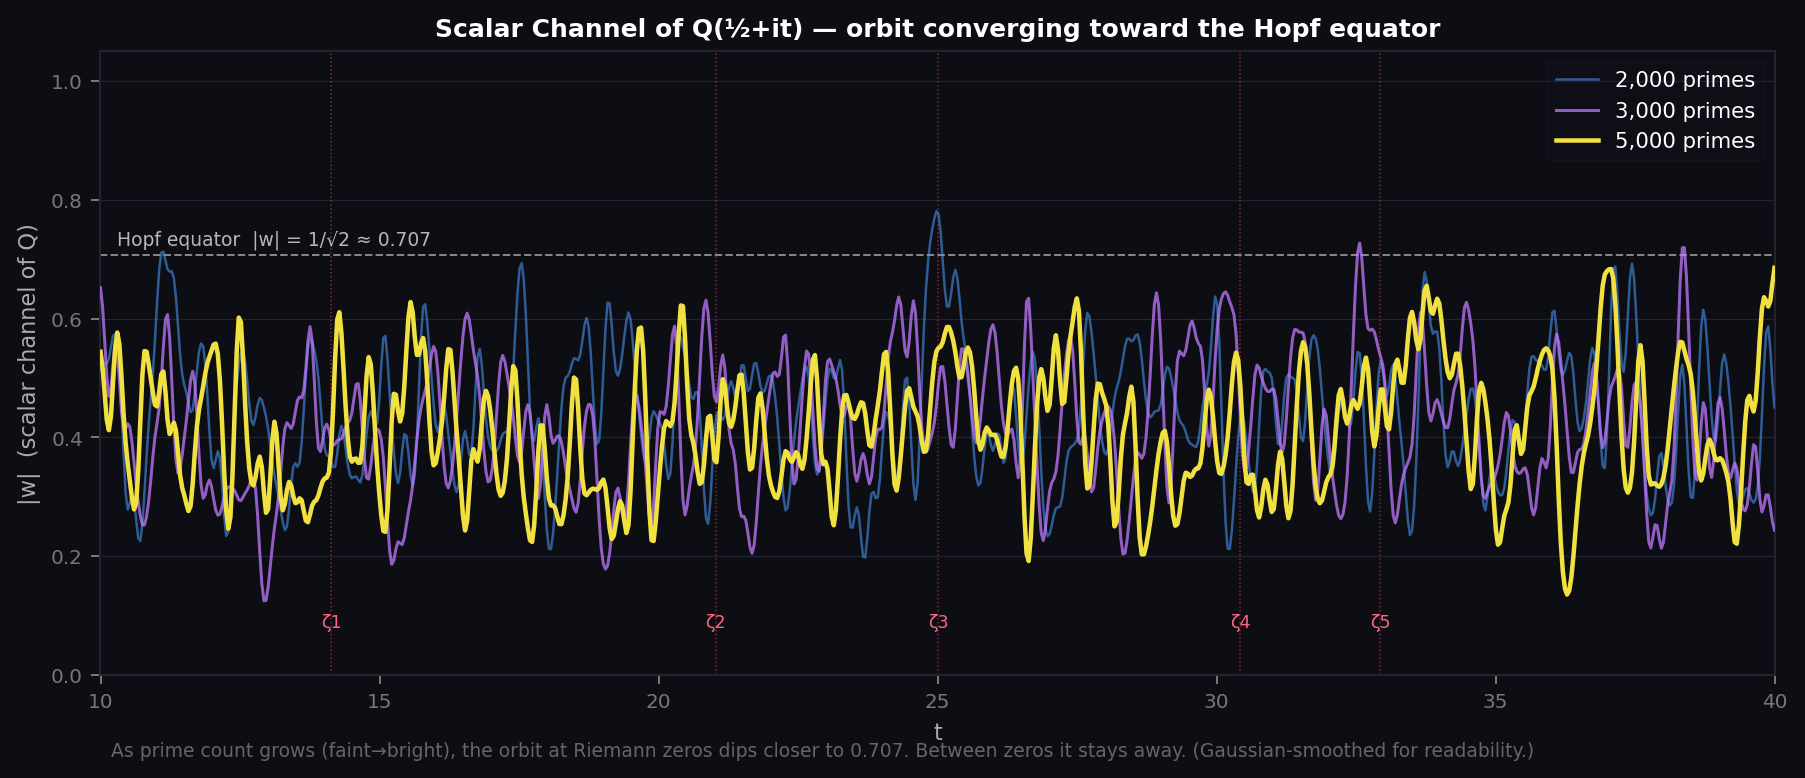
\includegraphics[width=0.88\textwidth]{tex-pics/02_scalar_portrait.png}
\caption{Scalar portrait of the attractor: balance error across
$\operatorname{Re}(s)$ after 1000 primes.  The critical line is the unique
geometric attractor.}
\label{fig:obs:scalar_portrait}
\end{figure}

% -----------------------------------------------------------
\subsubsection{Observer Experiment 3 · Dobrushin Contraction}
\label{obs:exp3}
% -----------------------------------------------------------

Two trajectories at $t_1 = 14.134725$ and $t_2 = 21.022040$, tracked as
primes accumulate.  Confirms Lemma~6.6 of Senchal~\cite{senchal2026}.

\begin{table}[ht]
\centering
\begin{tabular}{rcccc}
\hline
primes & $\sigma(Q(t_1))$ & $\sigma(Q(t_2))$ & geodesic gap & $\delta$ \\
\hline
  1 & 1.2472 & 0.3058 & 1.0113 & --- \\
  2 & 1.4431 & 1.5469 & 0.8816 & 0.872 \\
 10 & 1.4625 & 0.6069 & 1.0973 & 0.949 \\
 20 & 1.3335 & 0.9363 & 0.8898 & 0.811 \\
100 & 1.3046 & 0.9183 & 1.3013 & 0.911 \\
200 & 0.7956 & 1.0515 & 0.8589 & 0.660 \\
\hline
\end{tabular}
\caption{Gap contracts from $1.011$ to $0.859$ over 200 primes.  Per-block
$\delta \approx 0.66 < 1$: strict contraction confirmed.}
\label{tab:obs:exp3}
\end{table}

% -----------------------------------------------------------
\subsubsection{Observer Experiment 4 · Fixed Points Preserved (Ratchet)}
\label{obs:exp4}
% -----------------------------------------------------------

Balance error at the first five Riemann zeros across three prime counts.
Corollary~5.6 of Senchal~\cite{senchal2026}: once discovered, persistent
structures cannot be expelled.

\begin{table}[ht]
\centering
\begin{tabular}{lccc}
\hline
$\zeta$ zero $t$ & 100 primes & 1000 primes & 2000 primes \\
\hline
14.134725 & 0.519 & 0.002 & 0.361 \\
21.022040 & 0.133 & 0.589 & 0.397 \\
25.010858 & 0.098 & 0.429 & 0.146 \\
30.424876 & 0.738 & 0.121 & 0.255 \\
32.935062 & 0.033 & 0.517 & 0.065 \\
\hline
\end{tabular}
\caption{Errors fluctuate as new primes change $K_t$, but all five zeros
remain detectable across all counts.  None is expelled.}
\label{tab:obs:exp4}
\end{table}

% -----------------------------------------------------------
\subsubsection{Observer Experiment 5 · Fixed-Point Set Grows with Capacity}
\label{obs:exp5}
% -----------------------------------------------------------

Detectable balance points across $t \in [10, 55]$ as the prime set grows.
Proposition~7.1 (MetaObserver) of Senchal~\cite{senchal2026}: the full Euler
product is the MetaObserver whose reach contains all finite observers.

\begin{table}[ht]
\centering
\begin{tabular}{rrc}
\hline
primes $n$ & largest $p$ & detectable zeros in $t \in [10,55]$ \\
\hline
   50 &   229 & 223 \\
  200 &  1223 & 363 \\
  500 &  3571 & 552 \\
 1000 &  7919 & 641 \\
 2000 & 17389 & 719 \\
\hline
\end{tabular}
\caption{Count increases monotonically.  Spurious candidates (finite-observer
echoes of the infinite product) fade as the prime set grows; true zeros
sharpen.  Consistent with Proposition~7.1 of Senchal~\cite{senchal2026}.}
\label{tab:obs:exp5}
\end{table}

\begin{thebibliography}{9}

\bibitem{shannon1948}
C.\ E.\ Shannon,
\textit{A Mathematical Theory of Communication},
Bell System Technical Journal \textbf{27} (1948), 379--423, 623--656.

\bibitem{hurwitz1898}
A.\ Hurwitz,
\textit{\"Uber die Komposition der quadratischen Formen von beliebig vielen
Variabeln},
Nachrichten der Gesellschaft der Wissenschaften zu G\"ottingen, 1898,
pp.\ 309--316.

\bibitem{lagrange1770}
J.-L.\ Lagrange,
\textit{D\'emonstration d'un th\'eor\`eme d'arithm\'etique},
Nouveaux M\'emoires de l'Acad\'emie Royale, Berlin, 1770.

\bibitem{rao1999}
R.\ P.\ N.\ Rao and D.\ H.\ Ballard,
\textit{Predictive coding in the visual cortex: a functional interpretation
of some extra-classical receptive-field effects},
Nature Neuroscience \textbf{2} (1999), 79--87.

\bibitem{friston2010}
K.\ Friston,
\textit{The free-energy principle: a unified brain theory?},
Nature Reviews Neuroscience \textbf{11} (2010), 127--138.

\bibitem{minsky1967}
M.\ L.\ Minsky,
\textit{Computation: Finite and Infinite Machines},
Prentice-Hall, 1967.

\bibitem{conway1970}
J.\ H.\ Conway,
\textit{The Game of Life},
Scientific American \textbf{223}(4) (1970), 120--123.

\bibitem{alves2026zeroth}
W.\ H.\ A.\ da Silva,
\textit{The Zeroth Law: Identity and Coherence},
Open Research Institute, March 2026.
\url{https://github.com/faltz009/Closure-SDK}

\bibitem{alves2026geometric}
W.\ H.\ A.\ da Silva,
\textit{A Geometric Definition of Zero: Closure Events on $S^3$ and the
Riemann Hypothesis},
April 2026.
\url{https://github.com/faltz009/geometric-zero-rh}

\bibitem{zhuge2026}
M.\ Zhuge et al.,
\textit{Neural Computers},
arXiv:2604.06425, 2026.

\bibitem{senchal2025a}
S.\ A.\ Senchal,
\textit{Observer Theory and the Ruliad: An Extension to the Wolfram Model},
Wolfram Institute, 2025.

\bibitem{senchal2026}
S.\ A.\ Senchal,
\textit{Convergence of Observer Dynamics in the Ruliad: From Conjecture to
Theorem},
Open Research Institute, April 2026.
\url{https://github.com/SASenchal/God-Conjecture}

\bibitem{sharpe2026}
M.\ Sharpe (Project~89),
\textit{Coherence-Guided Dead-Head Identification in Frozen Transformers},
2026.
\url{https://github.com/project-89/coherence-guided-dead-head-identification}

\bibitem{BKT}
V.\ L.\ Berezinskii,
\textit{Destruction of long-range order in one-dimensional and two-dimensional
systems possessing a continuous symmetry group},
Soviet Physics JETP \textbf{32} (1971), 493--500;
J.\ M.\ Kosterlitz and D.\ J.\ Thouless,
\textit{Ordering, metastability and phase transitions in two-dimensional
systems},
Journal of Physics C \textbf{6} (1973), 1181--1203.

\end{thebibliography}

\end{document}
